%-------------------------------------------------------------------
%-------------------------------------------------------------------
%----------------------   BA Andreas Korb   ------------------------
%-------------------------------------------------------------------
%-------------------------------------------------------------------


%%%%%%%%%%%%%%%%%%%%%%%%%%%%%%%%%%%%%
%%%%%%%%%%%%  Preamble  %%%%%%%%%%%%
%%%%%%%%%%%%%%%%%%%%%%%%%%%%%%%%%%%%%
\documentclass[
	11pt,			%Font size
	a4paper,		%Sheet size
	DIV=12,			%Type area (division into boxes)
	parskip=half,	%No indentation but line spacing for new paragraph
	headsepline,	%For dividing line on head side
	openany,        %Allow chapter to start on any page (even or odd)
	bibliography=totoc,  %Add References to table of contents
	listof=totoc   %Add List of Figures to table of contents
]{scrbook}

%Todo Randausgleich

% No additional spacing in front of chapter heading
\RedeclareSectionCommand[
  beforeskip=0pt
]{chapter}

%Cross-platform
\usepackage[utf8]{inputenc}

%Font coding
\usepackage[T1]{fontenc}

%German Umlauts / Coding / Hyphenation
%\usepackage[ngerman]{babel}

%improved edge compensation
\usepackage{microtype}

%Code highlighting
\usepackage{float}
\usepackage[newfloat]{minted}

\usepackage[hidelinks]{hyperref}

%Embed references
\usepackage{csquotes}
\usepackage[svgnames]{xcolor}
\definecolor{thi}{RGB}{0,90,155}
\hypersetup{
	colorlinks,
	linkcolor={thi},
	urlcolor={thi},
	citecolor={thi},
}

% sorting=none that they appear in the order they're used
\usepackage[sorting=none, sortcites]{biblatex}

\addbibresource{references.bib}

%Set font
%Default cmr10 --> Computer Modern Roman 10pt (stored as bitmap)
\usepackage{lmodern}	%Vector version of cmr10

%\renewcommand{\familydefault}{\sfdefault}	%sf --> Without serifs

%Embed fonts
\usepackage{graphicx}
\usepackage{import}
\graphicspath{{images/}}

%Embed maths
\usepackage{amsmath,amssymb}

%Improved table display
\usepackage{booktabs}

%Display table and figures next to text
\usepackage{wrapfig}

\author{Andreas Diemo Korb\vspace{9ex}}
\title{Evaluating approaches for more efficient UDS protocol scanning}
\subtitle{\vspace{1.5ex} to obtain the academic degree Bachelor of Science\vspace{3ex}}

\date{}

%Information on the bottom side of the cover sheet
\publishers{
	\begin{tabular}{rl}
		\textbf{Study program}	    & Bachelor Computer Science \\ 
		\textbf{Faculty}		    & Computer Science \\
		\textbf{Issue date}	        & \today \\
		\vspace{6ex}
	\end{tabular}
	
	\begin{tabular}{rl}
		\textbf{First supervisor}	& Prof. Dr. Hans-Michael Windisch \\
		\textbf{Second supervisor}	& Prof. Dr. Ulrich Margull \\
		\textbf{External supervisor}& Lukas Lisowski \\
		\textbf{External company}	& eMundo GmbH
	\end{tabular} 
}


%Header and footer
\usepackage[automark,footsepline,plainfootsepline]{scrlayer-scrpage}
\pagestyle{scrheadings}
\clearpairofpagestyles
\ihead{\leftmark}
\ifoot{Andreas Korb}
\ofoot*{\pagemark}

%THI Logo at the beginning of the cover page
\titlehead{
	\hfil	%Horizontal gap
	
\includegraphics[width=0.3\textwidth]{thi_logo_cropped}   \hspace*{3cm}
\includegraphics[width=0.3\textwidth]{emundo}
	\hfil
}

% begin appendix autoref patch [\autoref subsections in appendix](https://tex.stackexchange.com/a/149897)
\usepackage{appendix}

\def\sectionautorefname{Section}
\def\subsectionautorefname{Section}
\def\subsubsectionautorefname{Section}
\def\appendixautorefname{Appendix}

\usepackage{etoolbox}
\makeatletter
\patchcmd{\hyper@makecurrent}{%
    \ifx\Hy@param\Hy@chapterstring
        \let\Hy@param\Hy@chapapp
    \fi
}{%
    \iftoggle{inappendix}{%true-branch
        % list the names of all sectioning counters here
        \@checkappendixparam{chapter}%
        \@checkappendixparam{section}%
        \@checkappendixparam{subsection}%
        \@checkappendixparam{subsubsection}%
        \@checkappendixparam{paragraph}%
        \@checkappendixparam{subparagraph}%
    }{}%
}{}{\errmessage{failed to patch}}

\newcommand*{\@checkappendixparam}[1]{%
    \def\@checkappendixparamtmp{#1}%
    \ifx\Hy@param\@checkappendixparamtmp
        \let\Hy@param\Hy@appendixstring
    \fi
}
\makeatletter

\newtoggle{inappendix}
\togglefalse{inappendix}

\apptocmd{\appendix}{\toggletrue{inappendix}}{}{\errmessage{failed to patch}}
\apptocmd{\subappendices}{\toggletrue{inappendix}}{}{\errmessage{failed to patch}}
% end appendix autoref patch

\providecommand*{\listingautorefname}{Listing}


\usepackage[acronym, toc, nogroupskip, style=long]{glossaries}
\usepackage{glossaries-extra}
\makeglossaries

\newacronym{can}{CAN}{Control Area Network}
\newacronym{ccp}{CCP}{CAN Calibration Protocol}
\newacronym{dsc}{DSC}{Diagnostic Session Control}
\newacronym{ecu}{ECU}{Electronic Control Unit}
\newacronym{gmlan}{GMLAN}{General Motors Local Area Network}
\newacronym{ip}{IP}{Internet protocol}
\newacronym{isotp}{ISOTP}{ISO transport protocol}
\newacronym{lin}{LIN}{Local Interconnect Network}
\newacronym{nr}{NR}{Negative response}
\newacronym{nrc}{NRC}{Negative response code}
\newacronym{obd}{OBD}{On-board diagnostics}
\newacronym{pr}{PR}{Positive response}
\newacronym{pets3}{PetS3}{Penetration Test Driven Safety and Security System Improvements for Cyber-Critical Systems}
\newacronym{rc}{RC}{Routine Control}
\newacronym{rdbi}{RDBI}{Read Data By Identifier}
\newacronym{sa}{SA}{Security Access}
\newacronym{sid}{SID}{Service identifier}
\newacronym{tcp}{TCP}{Transmission Control Protocol}
\newacronym{udp}{UDP}{User Datagram Protocol}
\newacronym{uds}{UDS}{Unified Diagnostic Services}


%%%%%%%%%%%%%%%%%%%%%%%%%%%%%%%%%%%%%%%%%
%%%%%%%%%%%%  Document begin  %%%%%%%%%%%
%%%%%%%%%%%%%%%%%%%%%%%%%%%%%%%%%%%%%%%%%
\begin{document}

\renewcommand{\thepage}{\roman{page}}% Roman page numbers

\maketitle
\thispagestyle{empty}

\addsec{Declaration}
\thispagestyle{plain}

I hereby declare that this thesis on the subject is my own work, that I have not presented it elsewhere for examination purposes and that I have not used any sources or aids other than those stated. I have marked verbatim and indirect quotations as such.
\vspace{3cm}

Ingolstadt, 08.03.2021


\setcounter{tocdepth}{1} 	% Table of contents only Chapters and Sections
\thispagestyle{plain}
\tableofcontents

\clearpage
\renewcommand{\thepage}{\arabic{page}}% Arabic page numbers

\section{Introduction}

\subsection{Motivation}
Nowadays a car is full of small computers handling tasks for the whole system. Without these helpers, functions like driver-assistance or self-diagnostic would not be possible. Those computers are generally called electronic control unit (ECU). Modern cars can contain over 100 of those. The complexity of ECU networks in a car is increasing quickly. The next generation of car networks is expected to be more centralized with less ECUs \cite{car-architecture}. This reduces complexity and its inherent risk of security vulnerabilities and high costs, as shown in \autoref{fig:centralized-architecture}.

%durations
\begin{figure}[h]
    \centering
    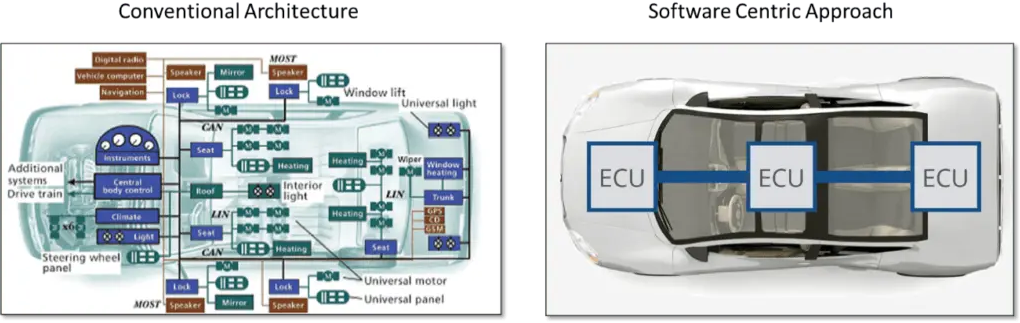
\includegraphics[width=1\textwidth]{centralized-architecture}
    \caption{Illustration of the current and the next-gen architecture of cars \cite{car-architecture}.}
    \label{fig:centralized-architecture}
\end{figure}

ECUs communicate with each other via bus systems. The most common ones are CAN, FlexRay and the Automotive Ethernet, which is becoming increasingly popular. Transport protocols usually sit on top of these physical layers. For Ethernet this is the well known TCP protocol, while the most common one for CAN is the ISO-TP protocol. Application protocols are used to ultimately transfer payload. For example, some protocols were created specifically for the development of units like Universal Measurement and Calibration Protocol (XCP) and some others were defined for diagnostic purposes such as Unified Diagnostic Services (UDS), General Motors Local Area Network (GMLAN) and On-board diagnostics (OBD). Both types are security critical. The XCP protocol is able to read and even write into the flash memory of an ECU. It shall be disabled on shipped ECUs. The UDS and GMLAN protocol provide definitions for diagnostic related tasks. However, diagnostic protocols are explicitly designed for actively used cars and thus exposed to the easily accessible OBD-II port, which by regulation must be present near the steering wheel on at least every car built after 2003 (see \autoref{fig:obd-port}). This fact makes them a great first target for gathering information. This work puts the UDS protocol in focus since it is the widest adopted protocol which allows extended functionality, for example flashing ECUs. The OBD protocol is excluded in this work because it does not offer any valuable information and the GMLAN protocol because it is restricted to vehicles from the General Motors corporation.

\begin{figure}[h]
    \centering
    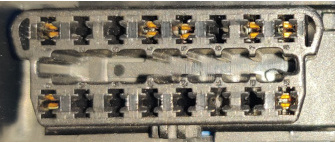
\includegraphics[width=0.5\textwidth]{obd-port}
    \caption{The OBD-II port of a BMW.}
    \label{fig:obd-port}
\end{figure}

The initial step in testing a system for weaknesses is to gather as much information from it as possible. In most cases, a protocol definition does not require that its specifications is fully supported; instead, a subset is sufficient.
Furthermore, a diagnostic protocol can define various states. The ECU may show varying behaviors in different states, for example support for other services. Since this kind of information is highly relevant for the security of the ECU, it would be helpful for security testers to gain this knowledge quickly and automatically.

One option to achieve this is to send all possible requests to an ECU and evaluate the responses. In the context of the project \emph{Penetration Test Driven Safety and Security System Improvements for Cyber-Critical Systems} (PetS3) \cite{pets3} such scanners have been implemented for UDS, GMLAN and OBD.

With their brute-force approaches, they are effective but not efficient. A scan can take a highly variable amount of time. It can range from a few hours to a day or more. In general, the more states are found on an ECU in a scan, the more time it will need. For example, more authentication information leads to more state detections and thus to higher runtimes. In addition, the response time of the ECU is also a decisive factor. The original runtimes observed of one UDS scan on the available ECUs are shown in \autoref{fig:durations} generated with the \mintinline{text}{plotly} library \cite{plotly}. It should be noted, that these scans have been executed with no additional information about the ECU as well. Accordingly, only the states that can be found without further information were detected.

%durations
\begin{figure}[h]
    \centering
    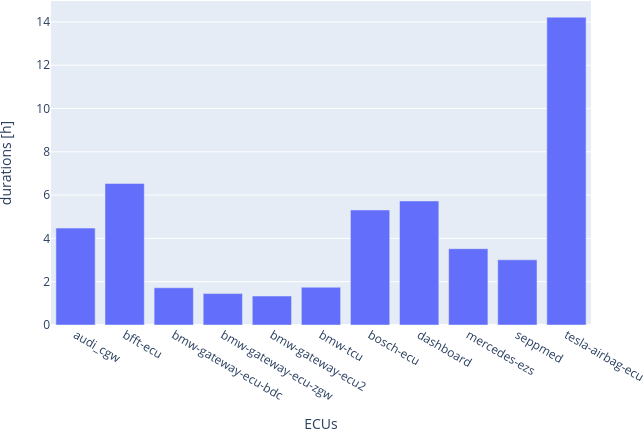
\includegraphics[width=1\textwidth]{durations}
    \caption{Observed runtimes for one UDS scan.}
    \label{fig:durations}
\end{figure}

Consequently, an efficient scan is desirable that keeps the scan time low even though many states can be found or the ECU has a high response time.

\subsection{Goal}

This paper evaluates different approaches to improve the efficiency of the UDS protocol scanning. The approaches can be mixed freely, if this leads to better results.

Efficiency improvement is understood as the ratio between the speed-up and the coverage. Coverage is here defined as the ratio of finds in the unmodified Scanner to the finds of the modified Scanner, and the speed-up as the saved time in comparison between these two. For both metrics, the higher the better.

Nevertheless, the coverage and speed-up have to be in balance. A speed-up of 90\% is not helpful if this results in 0\% coverage. The speed-up is achieved by reducing the number of generated packets. Hence, the challenge is to narrow down the scanning area to where positive responses are expected.


\subsection{Environment}
This work was created at eMundo GmbH in Ingolstadt. It is an IT service company which plans and executes projects for customers. Also, it is an aspiring company which in 20 years managed to open in total six company headquarters in Germany, Austria and Italy with almost 100 employees.

Since 2018, they are part of the \emph{Penetration Test Driven Safety and Security System Improvements for Cyber-Critical Systems} (PetS3) project. It is a collaboration research project among the OTH Regensburg, TH Nürnberg, EDAG Engineering Group AG, sepp.med GmbH, intive automotive GmbH and eMundo GmbH.

Due to the advancing networking, cyberattacks are a growing threat to a variety of application areas such as connected vehicles or smart metering. Common concepts of functional safety and IT security are required for these gateway-based systems. The aim of the research project is to investigate attacks on the IT security of system architectures of networked cyber-critical systems, since the interaction between functional safety and IT security is largely unknown in this context.

This paper is the final result of this project on the part of eMundo.

\subsection{Outline}

\section{Background}

This section will explain the technical fundamentals which are necessary to understand the full bachelor thesis.

\subsection{The Scapy program}
\label{sec:scapy}

%UDS stack
\begin{wrapfigure}{r}{0.15\textwidth}
    %
\includegraphics[width=0.1\textwidth]{scapy_logo}
    \raisebox{0pt}[\dimexpr\height-1.5\baselineskip\relax]{
\includegraphics[width=0.15\textwidth]{scapy_logo}}
    %\label{fig:scapy-logo}
\end{wrapfigure}

The homepage of Scapy introduces itself with \cite{scapy}:
\begin{displayquote}
Scapy is a powerful interactive packet manipulation program. It is able to forge or decode packets of a wide number of protocols, send them on the wire, capture them, match requests and replies, and much more.
\end{displayquote}

So, it fulfills the requirements of protocol scanners:
\begin{itemize}
    \item Receiving and transmitting packets
    \item Support for many physical layers and transport protocols
    \item Simple definition of packet structures
    \item Matching requests with their responses
\end{itemize} 

It is used through a text-based user interface. This has the advantage of being lightweight, and working via ssh connections out-of-the-box. While being mainly a program, it can also be used as a library by importing the necessary classes and interfaces into the own Python program.

It supports Python 3 and also Python 2, even though its support has ended on 1st of January 2020. The following quote from a maintainer explains why \cite{scapy-py2}:

\begin{displayquote}
    Scapy is a tool that can be used in a very large number of situations. Often, you don't get to choose the Python interpreter you have when you run Scapy. So, [...] we need to keep supporting Python 2.7 as long as we can.
\end{displayquote}


\subsection{The CAN bus}

All communication performed and recorded in this paper with an ECU is done via the Control Area Network bus (CAN).

 Its specification is released in the ISO 11898. Each packet on this bus can transmit up to 8 bytes of payload and has an identifier which a length of either 11 or 29-bits, the former being more common. An identifier does not necessarily have to designate a physical device; it can also indicate one of several software modules of a device.
 The maximum data rate is 1 Mbit/sec with a network length below 40 m. The higher the length, the lower the possible data rate, as can be seen in \autoref{tab:can-speed}.

\begin{table}[h]
    \centering
    \begin{tabular}{ccc}
    \hline
    \textbf{Bus Length (m)} & \textbf{Signaling Rate (Mbps)}\\
    \hline
    40 & 1 \\
    100 & 0.5 \\
    200 & 0.25 \\
    500 & 0.10 \\
    1000 & 0.05 \\
    \hline
\end{tabular}
\caption{Suggested Cable Length vs Signaling Rate \cite{slla270}.}
\label{tab:can-speed}
\end{table}

\subsubsection{Advantages for the automotive domain}

This bus is robust because it uses two lines of differential signals for communication. This means that if one wire is driven high, the other one is driven low. Thus, the receiver can reliably detect interferences by comparing these signals.

Moreover, CAN busses are using the bus network topology (see \autoref{fig:with-without-can}). This results in a smaller number of wires compared to star topologies, resulting in lower weight, which is an important factor for manufacturers.

%with-without-can
\begin{figure}[h]
    \centering
    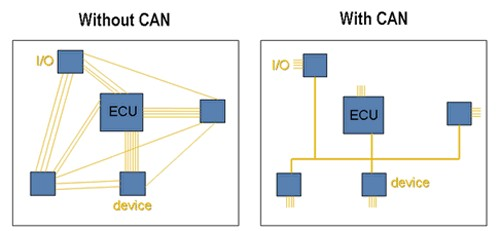
\includegraphics[width=0.7\textwidth]{with-without-can}
    \caption{CAN effect on decreasing the wire quantity \cite{Sharma2016}.}
    \label{fig:with-without-can}
\end{figure}

Last but not least, an important feature for the automotive application domain is the priority support. The lower the identifier, the higher the priority. Hence, if ECU1 and ECU2 transmit a CAN packet at exactly the same time, the packet with the lower identifier wins, the other one is discarded and will be retransmitted. This is called the Carrier Sense Multiple Access with Collision Detection (CSMA/CD) protocol \cite{Sharma2016}. For this reason, diagnostic CAN identifiers tend to have a high identifier \cite{Herrewegen2018}.

\subsubsection{Security vulnerabilities}

Thinking this one step further, CAN is vulnerable to denial of service attacks. This attack can be performed by flooding the CAN bus with zero-identifier messages resulting in drops of legitimate packets \cite{Buttigieg2017}.

Furthermore, Buttigieg et al. \cite{Buttigieg2017} describe three more security issues of the CAN bus protocol in their paper {Security Issues in Controller Area Networks in Automobiles}.
First, CAN packets do not contain any authentication information. An ECU receiving a message is not able to distinguish between a message from a legitimate ECU and a malicious one \cite{Buttigieg2017}. So, for example, if the state of an ECU is changed to a higher privileged state, all devices, including malicious ones, will have access to its newly unlocked services and information. Countermeasures exist in the form of performing authentication, but there is no satisfying solution yet, which fulfills cost-effectiveness, backward compatibility, support for vehicle repair and maintenance, sufficient implementation details, and acceptable overhead \cite{Bozdal2020}.
Also, originally, CAN bus networks lacked network segmentation, since each message is broadcasted and received by each node of the network \cite{Buttigieg2017}. Nowadays, car networks of higher-class cars like Audi and BMW are usually divided into less and more critical segments by so-called Gateway ECUs \cite{Bozdal2020}. Despite the increase in the level of security, this makes it more difficult to maintain the system, which is associated with increased costs \cite{Bozdal2020}.
The final security vulnerability is the lack of data encryption \cite{Buttigieg2017}. Lightweight encryption systems could be implemented, but are limited by the short length of the data field (8 bytes) and the limited computing power of ECUs \cite{Bozdal2020}.

Since all countermeasures described in the previous paragraph are limited, Intrusion Detection Systems (IDS) are emerging, with the advantages of not having to change the current CAN controller and not increasing bus traffic \cite{Bozdal2020}. Such a system has been implemented in the context of the PetS3 project \cite{spahn2018}.

\subsubsection{Virtual CAN interfaces and using the can-utils}
\label{subsubsec:can-utils}

Virtual CAN interfaces can be used for simulations or simple tests. They are supported natively by Linux without additional actions.
To create a virtual CAN interface, only one command in a Linux shell is required:
\begin{minted}{text}
sudo ip link add vcan0 type vcan
\end{minted}

The most common tool set to work with the CAN bus are the can-utils \cite{can-utils}, which can be usually installed with the package manager of the distributions. For example, the following command displays all messages of the CAN bus on interface \mintinline{text}{vcan0} in a terminal:
\begin{minted}{text}
candump vcan0
\end{minted}

Adding the \mintinline{text}{-l} option changes the output to be more compact instead of human-readable and stores the received traffic in a \mintinline{text}{candump.log} file:

\begin{minted}{text}
candump -l vcan0
\end{minted}

All traffic recorded in this work was done with this command.

For sake of completeness, this command sends a CAN packet with the identifier 0x123 and the payload \mintinline{text}{0x01 0x02}:
\begin{minted}{text}
cansend vcan0 123#01.02
\end{minted}

\subsection{The ISO-TP transport protocol for CAN}

CAN packets have a payload size of 8 bytes. This is sufficient for most UDS requests, but not for many UDS responses. Thus, ISO-TP is used as the transport protocol on the CAN bus for UDS communication.

It is defined in ISO 15765-2 and increases the payload size from 8 bytes to 4095 bytes per message. At least one byte of each CAN packet is then transport protocol information, indicating whether this packet is a single frame or if it only contains a fragment of the actual payload.

\subsection{The UDS protocol}

UDS stands for \emph{Unified diagnostic services} and is an application protocol defined in ISO 14229. This protocol defines the structures of request and response packets for diagnostic purposes sent over an arbitrary data link \cite{iso14229}.

The reason for the development of such a protocol was that the cars developed in the last decades were more and more able to diagnose themselves. A car repair shop only had to request this information from the car. But since there was no universal standard, car manufacturers tended to implement company-specific protocols for this purpose. UDS is an international standard and not company-specific, the \emph{Unified} in its name underlines this. 

%UDS stack
\begin{figure}[h]
    \centering
    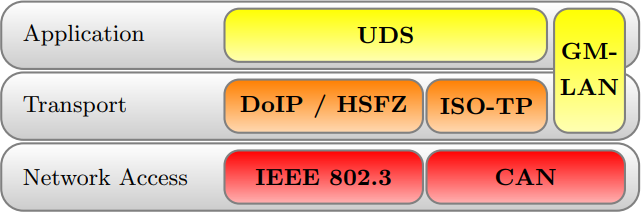
\includegraphics[width=0.7\textwidth]{uds-stack}
    \caption{The most common protocol stack for UDS \cite{Weiss2020}.}
    \label{fig:uds-stack}
\end{figure}

As shown in \autoref{fig:uds-stack}, the most common data links for the UDS protocol are the Ethernet and the CAN bus. Others can and are used as well, explicitly stated in the UDS standard are FlexRay, K-Line and LIN.

\subsubsection{Packet structure}

\begin{figure}[h]
    \centering
    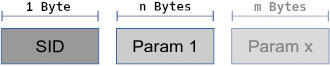
\includegraphics[width=0.5\textwidth]{uds-structure}
    \caption{The structure of UDS requests.}
    \label{fig:uds-structure}
\end{figure}

\autoref{fig:uds-structure} shows how UDS requests are structured. Each service is identified by a Service Identifier (SID). This identifier is the first byte of each UDS packet. It must not be confused with the identifier of the CAN packet. Then at least one parameter follows. Most common is only one parameter. But services with multiple parameters exist too.
Negative responses have the SID 0x7f.
For positive responses it is defined as 0x40 added to the SID. Thus, a request with SID 0x27 would be responded with 0x27 + 0x40 = 0x67 (see \autoref{fig:key-seed}).

\subsubsection{Services}
\label{subsubsec:uds-services}

UDS defines various services with different purposes. The ones used later in this paper are explained here.

The Routine Control (RC) service allows managing predefined routines on the ECU. They can be started, stopped or their results requested. It has two parameters, namely the desired action and the identifier of the routine.

Another service is called Read Data By Identifier (RDBI). With this service, it is possible to retrieve one or more values of a control unit. This can be static information like the software version or dynamic values such as the current readings of sensors. The structure of its requests is simple as it only contains an identifier as parameter.

The Diagnostic Session Control (DSC) service is used to enable different diagnostic states in the ECU, and the Security Access (SA) service to unlock restricted access to data or services. They are explained in more detail in the next section, as they affect the state of ECUs.

\subsubsection{States}
\label{subsec:states}

There is always exactly one global UDS state active for an ECU. It influences the behavior of the ECU and can be changed by sending specific requests. Just a few services are able to accomplish this. For example, sending a request with the SA or DSC service to the ECU may affect its state. Whether the ECU has actually changed the state can be easily determined by checking whether the sender received a positive or negative response.

\begin{figure}[h]
    \centering
    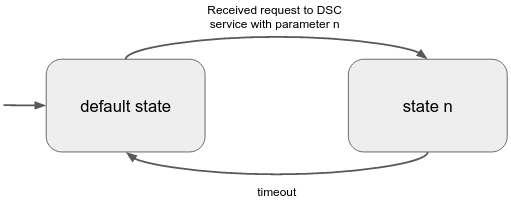
\includegraphics[width=0.7\textwidth]{ecu-state-behavior}
    \caption{State machine example of ECUs for UDS with the DSC service.}
    \label{fig:ecu-state-behavior}
\end{figure}

The default state is the active state after the ECU is switched on. Without an external request, it remains in this state. \autoref{fig:ecu-state-behavior} illustrates the behavior of the ECU when a request is received for the DSC service and parameter value $n$. In the DSC service, each parameter value specifies a state. Thus, if the ECU designers integrated a state for $n$, the controller will respond positively. It will now remain in this state until there has been no UDS communication for usually five seconds, then it will automatically return to the default state. If the ECU designers did not integrate such a state, it will answer with a negative response and remain in its current state.

The Security Access service uses the challenge–response authentication, in automotive terminology called seed-key protocol. The ECU sends a randomly generated value (the seed) to the client. Both devices generate a response (the key) based on the seed and the client sends its response to the ECU. If the keys match for the received and the generated response for the ECU, the client is authenticated \cite{iso14229}.

\begin{figure}[h]
    \centering
    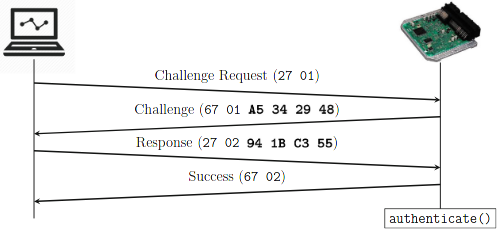
\includegraphics[width=0.7\textwidth]{key-seed}
    \caption{The challenge-response protocol \cite{Herrewegen2018}.}
    \label{fig:key-seed}
\end{figure}


\subsection{The UDS Scanner}

The UDS Scanner was implemented in Scapy for the PetS3 project.

\subsubsection{Purpose}

\begin{figure}[h]
    \centering
    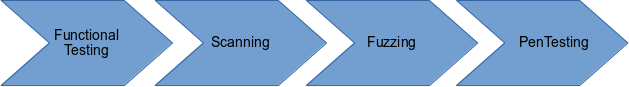
\includegraphics[width=0.8\textwidth]{automotive-security-testing-process}
    \caption{The Automotive Security Testing process.}
    \label{fig:automotive-security-testing-process}
\end{figure}

As \autoref{fig:automotive-security-testing-process} shows, the security testing process in the automotive domain contains a scanning step that aims to detect what services of a protocol are implemented and what information can be retrieved there \cite{Bayer2015}. The UDS Scanner fulfills these tasks. It can also be used for fuzzing, even though scanning is its main use-case. The retrieved information answers the following questions:

\begin{itemize}
\item Which services are supported?
\item What information can be read with these services?
\item What control options does the ECU offer?
\item Which states does it have, how does it behave in each?
\end{itemize}


\subsubsection{Procedure}

The UDS Scanner starts with scanning each service for the default state of the ECU (see \autoref{subsec:states}). While doing so, it detects new states, which will be scanned subsequently. So as long as new states are found during an iteration, the scan continues. After each iteration, the ECU is reset to return to the default state. Now, the next state to be scanned is activated by sending a sequence of UDS requests, which is an edge of the UDS Scanner's internally built state machine. An ECU reset is usually done by switching off the ECU, waiting a few seconds, and switching it on again, although there is an ECUReset service in the UDS protocol. However, its specification states that the behavior is implementation-specific, so a power-based reset is the cleaner way.

The following pseudocode aims to make the procedure easier to understand:

\begin{samepage}
\begin{minted}{python}
class UDS_Scanner:
    def scan():
       states = [default_state]
       for state in states:
           ecu.reset()
           ecu.enter_state(state)
           for service in service_list:
               service.scan() # detects new states
       ecu.reset()
\end{minted}
\end{samepage}

\section{Data gathering and profiling}
\label{sec:data-gathering}

From here, the procedure and the environment of gathering information to elaborate approaches is described.

\subsection{Remote test environment}

In order to find scan ranges that are likely to be answered positively, data from as many ECUs as possible is needed. In the context of the PetS3 project a remote testing environment has been created. This was particularly helpful in light of the contact limitations at the time of writing.

The infrastructure of Laboratory for Safe and Secure Systems (LaS3) was used for that. Specifically, their GitLab server was used, displayed in \autoref{fig:gitlab-screenshot}.

%GitLab screenshot
\begin{figure}[h]
    \centering
    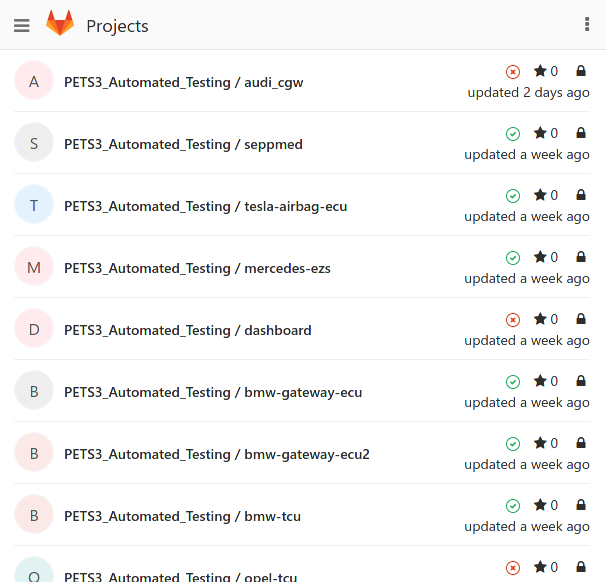
\includegraphics[width=0.7\textwidth]{gitlab-screenshot}
    \caption{Screenshot of the GitLab server.}
    \label{fig:gitlab-screenshot}
\end{figure}

Fourteen ECUs are available for testing on this server. However, three of them are from Opel and therefore only support GMLAN but not UDS.

For each ECU a YAML configuration file was created. Various work is done here, for example pulling and checking out the Scapy code from the currently working branch.

Then, the actual tests are executed that are written with the pytest framework. Here, a UDS scan can be started. At the same time, another process is started to record all CAN traffic that takes place during the execution of the tests.

Finally, the resulting files are uploaded to the GitLab server so that they can be downloaded via a browser program. Which files these are specifically and what they were used for will be explained in the next section.

\subsection{Explaining the generated data of a scan}

In total, four files are stored after a scan, which will be explained in this section.

\begin{itemize}
    \item candump.log
    \item generic.log
    \item profiling.csv
    \item data.pkl
\end{itemize}

\subsubsection{Record communication between scanner and ECU}

The resulting candump.log file recorded with the command explained in \autoref{subsubsec:can-utils} has a simple structure. Each line represents a CAN packet.

\begin{samepage}
\begin{minted}{text}
(<timestamp>) <interface> <identifier>#<payload>
(1611779255.926425) can1 714#03225FB2CCCCCCCC
(1611779255.929936) can1 77E#037F2231AAAAAAAA
(1611779255.935338) can1 714#03225FB3CCCCCCCC
(1611779255.940680) can1 77E#037F2231AAAAAAAA
\end{minted}
\end{samepage}

Unfortunately, these files contain a lot of information that is not only not needed, but also unwanted, as it leads to more difficult analysis because of higher storage and processing power usage. \autoref{fig:can-unwanted-information} shows the information that is not needed because it is ECU specific and does not add any value for the analysis.

%CAN unwanted information
\begin{figure}[H]
    \centering
    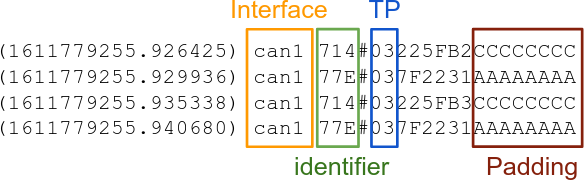
\includegraphics[width=0.7\textwidth]{can-unwanted-information}
    \caption{ECU specific information in candump.log.}
    \label{fig:can-unwanted-information}
\end{figure}

Consequently, an abstraction is desirable. The newly created format is called the generic format. It removes the interface, the padding, resolves the transport protocol information (ISO-TP) and replaces the identifier with representatives (s = Server, c = Client). Each line represents a UDS packet, instead of a lower layer CAN packet as in the candump logs. \autoref{fig:candump-generic-conversion} illustrates the input and output of a conversion.

%candump to generic conversion
\begin{figure}[h]
    \centering
    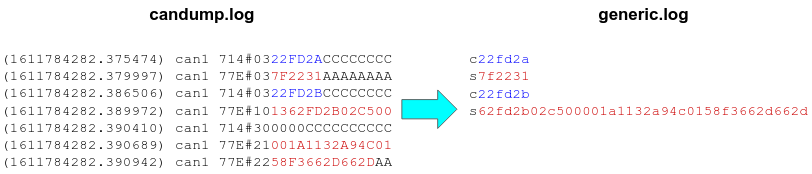
\includegraphics[width=1\textwidth]{candump-generic-conversion}
    \caption{candump.log to generic.log conversion.}
    \label{fig:candump-generic-conversion}
\end{figure}

This format proved to be very useful as it allows quick analysis by chaining common Linux programs.
For instance, counting the number of requests of a scan is a single command:
\begin{samepage}
\begin{minted}{bash}
        $ grep '^c.*' -c generic.log
        988844
\end{minted}
\end{samepage}

\subsubsection{Store service scan behavior of a scan}

For profiling, a file has been added as output to the UDS scanner, namely profiling.csv.

It contains which service scan ran under which state and when. It follows a fairly simple structure:

\begin{samepage}
    \begin{minted}{text}
        state     ,service  ,start            ,end
        ECU Reset ,ECU Reset,1611770228.135198,1611770228.658480
        [session1],CC       ,1611770228.661016,1611770231.236505
        ECU Reset ,ECU Reset,1611770231.236789,1611770231.754865
        [session1],DSC      ,1611770231.756320,1611770231.895722
    \end{minted}
\end{samepage}

Although an ECU Reset has no state, all occurrences of it get the same named state for better visualization of the log later.

\subsubsection{Store the finished scanner object}

Last but not least, the data.pkl file. Pickle is the object serialization module of the Python Standard library \cite{pickle}. The data.pkl file is the serialized UDS Scanner object after the scan and thus contains all the results, consisting of the responses for each request for each state of an ECU. This is helpful for debugging, analysis and also for simulation.


\subsection{Profiling the UDS Scanner}

The Pareto principle indicates that small number of causes can be responsible for a large percentage of effects \cite{pareto}. This is also applicable to optimization problems. Usually only a few number of code lines cause the majority of the runtime. Optimizing them is far more effective than performing micro-optimizations as they naturally improve the performance to a greater extent. Moreover, micro-optimizations are usually even more difficult to accomplish.

\subsubsection{Visualizing UDS scans}

To profile the UDS Scanner, the profiling.csv files is used. With its help Gantt charts are created which show the sequence and duration of the scanned services. This visualizes what parts of the UDS Scanner cause most of its runtime.

These charts have been created for each available ECU. For illustration one is sufficient since each showed the same gist (see \autoref{fig:tesla-gantt}).

\begin{figure}[H]
    \centering
    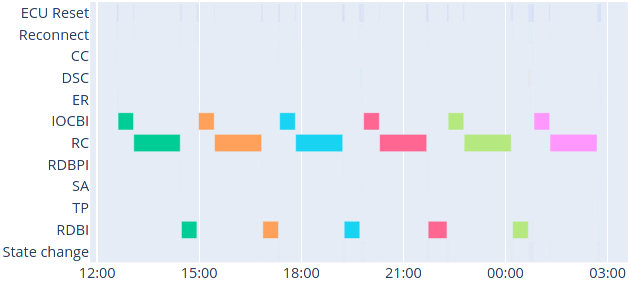
\includegraphics[width=0.9\textwidth]{tesla-gantt}
    \caption{Gantt chart of the Tesla-Airbag-ECU. Each color is a state.}
    \label{fig:tesla-gantt}
\end{figure}


\subsubsection{Identifying the services causing the most runtime}

Although it seems that some services and events do not require any time, their time consumption is only so small that they are not or hardly visible in this scaled-down version of the diagram.

The main cause of runtime is the RC service. This was expected, since this it requires the most requests for a complete scan.
In second place are the IOCBI and the RDBI service. They generate the same runtime, this was to be expected as well since they require the same number of requests. However, the IOCBI service is less frequently supported by ECUs than the RDBI service, resulting in a smaller runtime contribution when considering approach 3.

In summary, the RC and the RDBI service are the most critical runtime causes of the UDS scanner and therefore belong to the matters to be optimized.

\section{Elaboration of the realization of the approaches}

This section discusses the optimization of the two service scans from the previous section, each using a different approach. In addition, the third approach discussed is to avoid scanning unsupported services.

\subsection{Reuse information within same service}

This approach aims to reuse information from one part of a service for another part of this service. First, it must be checked to which service this approach should be applied to.

\subsubsection{Choosing the RC service to apply the approach to}

This approach is applicable to scans of services with multiple parameters, as it is the case for the Routine Control (RC) service. It has two parameters, the routine type and the routine identifier (more in \autoref{subsubsec:uds-services}). The distribution of the identifiers is visualized grouped by the type as a histogram in \autoref{fig:rc-distribution}.

\begin{figure}[h]
    \centering
    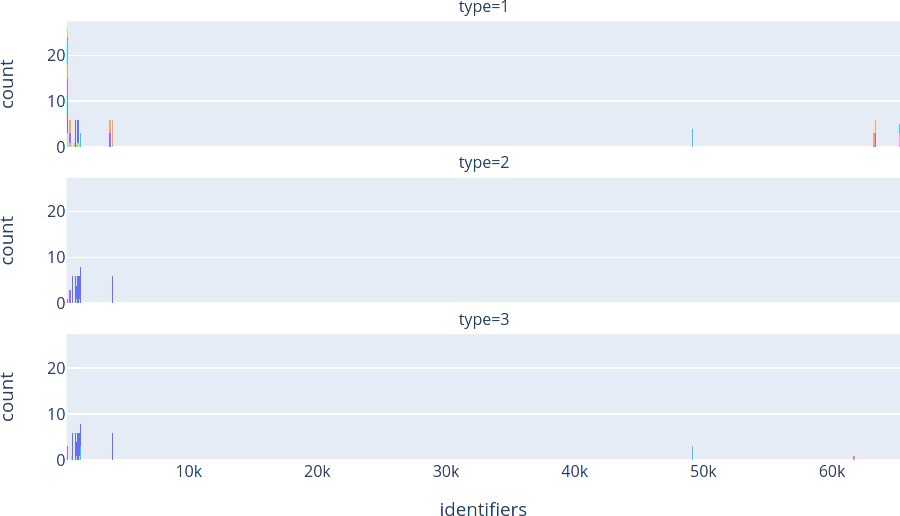
\includegraphics[width=0.8\textwidth]{rc-distribution}
    \caption{Distribution of the RC identifiers. Each color is one ECU.}
    \label{fig:rc-distribution}
\end{figure}

It can be seen that if an identifier is available in Type1, it is likely that this identifier also occurs in Type2 or Type3. Consequently, if an identifier does not respond positively in Type1, it is unlikely that it will respond in Type2 or Type3.

Hence, the RC service is a great candidate for this approach.

\subsubsection{Current behavior}

There are three control types, and because the identifier field has a length of 16-bits, there are 2\textsuperscript{16} identifiers. This leads to the following formula, showing how many requests are generated for a UDS scan:
\[f(n)=3 \cdot 2^{16} \cdot n\]
wherein $n$ stands for the number of detected states.

The current RC scan does exactly this, it generates the full range for each state. Its current behavior is illustrated in \autoref{fig:rc-behavior-current}. The green areas symbolize the scanned ranges.

\begin{figure}[h]
    \centering
    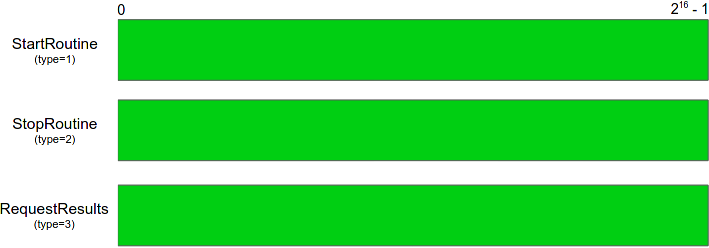
\includegraphics[width=0.8\textwidth]{rc-behavior-current}
    \caption{Current behavior of the RC service scan.}
    \label{fig:rc-behavior-current}
\end{figure}

\subsubsection{Elaborating the new behavior}
\label{subsubsec:rc-elaborating}

The new behavior starts with scanning all 2\textsuperscript{16} identifiers with Type1. Only the identifiers, which led to a positive response, are scanned with Type2 and Type3 as well. So, 2\textsuperscript{16} is the new minimum number of requests for each state for this service, resulting in an upper limit of request savings of 66.7 \%.

It was observed that there seems to be a locality effect for the identifiers. Thus, if an identifier with Type1 is answered positively, scanning also nearby identifiers for Type2 and Type3 results in higher coverage. To exploit this, an expansion width is introduced. This width specifies how a single value is expanded to a range in both directions. For example, with an expansion width of 100, the value 1500 would be expanded to the range 1400 – 1600.

\autoref{fig:rc-behavior-new} illustrates the new behavior. The green areas again show the scanned ranges. In addition, the red areas are the found identifiers in Type1 and their resulting scans for Type2 and Type3. The gray areas show the routine identifiers not requested with this new behavior.

\begin{figure}[h]
    \centering
    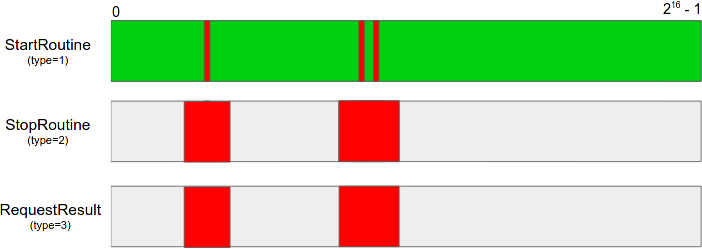
\includegraphics[width=0.8\textwidth]{rc-behavior-new}
    \caption{New procedure for scanning the RC service.}
    \label{fig:rc-behavior-new}
\end{figure}

What needs to be found out is the expansion width which leads to the best coverage, while maintaining an appropriate request saving. For this, scans with different expansion widths were simulated. These simulations work based on the information gathered from the real ECUs as described in \autoref{sec:data-gathering}. For a quick simulation another observation is used. If an identifier is available in a state, it is likely to be available in the other states too. Thus, the states are ignored in the simulation, which improves the performance by a multiple, while it is still close to the real ECUs. The required information, which identifiers are supported by an ECU for which type, is extracted from the generic.log files.

As described, the simulation starts with getting all identifiers which have been positively answered by the currently simulated ECU. Subsequently, these identifiers are expanded to both sites from 0 to 1000. Overlapping ranges are resolved to a continuous space. The sizes of the resulting ranges lead to the theoretically generated requests which can be calculated to the coverage and request saving. These values of all ECUs are averaged to the final result.
 
The following pseudocode shows the procedure more clearly.

\begin{samepage}
\begin{minted}{python}
coverages = []                                                 
speedups = []                                                  
for expansion_width in range(1000):                             
    coverages_ecus = []                                       
    speedups_ecus = []                                        
    for ecu in ecus:                                           
        ids_type1 = get_type1_ids(ecu)                         
        to_scan = ids_to_block(ids_type1, expansion_width)     
        coverages_ecus.append(get_coverage(ecu, to_scan))     
        count_requests = len(to_scan)                          
        speedups_ecus.append(get_speedup(ecu, count_requests))
    coverages[expansion_width] = avg(coverages_ecus)
    speedups[expansion_width] = avg(speedups_ecus)
\end{minted}
\end{samepage}

The result of this simulation is plotted in \autoref{fig:rc-simulation-result}. The request saving is almost linear to the expansion width. That makes sense, because the larger the expansions are, the more requests are generated. The expansion width of zero represents the results without using the locality effect.

\begin{figure}[h]
    \centering
    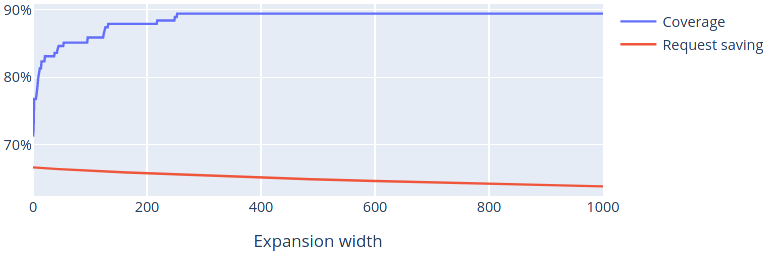
\includegraphics[width=0.7\textwidth]{rc-simulation-result}
    \caption{Result of the RC scan simulation to find the best expansion width.}
    \label{fig:rc-simulation-result}
\end{figure}

Since the request saving decreases only slowly, the highest coverage was chosen, which starts with the expansion width \textbf{253}. Hence, this value is the chosen and implemented one.

The simulations were also run with expanding identifiers in one direction only, which yielded very similar results. Thus, it was left in both directions.


\subsection{Use probabilities of positive answers block based}

Most services are simpler and only have one parameter. So, reusing information within the same service is not practical. This approach tackles these kinds of services. The new idea is to scan the blocks more heavily where positive behavior is more likely than others and vice versa.

\subsubsection{Choosing the RDBI service to apply the approach to}

The Read Data By Identifier (RDBI) service has only one parameter, the identifier of the requested data.

The distribution of positively answered identifiers over all ECUs is visualized in a histogram to check if there is potential. The result can be seen in \autoref{fig:rdbi-distribution}.

\begin{figure}[h]
    \centering
    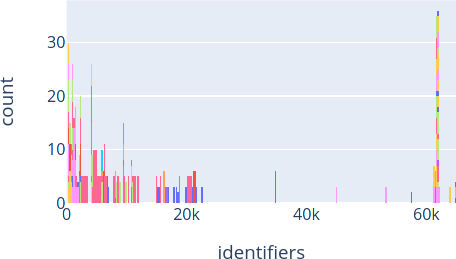
\includegraphics[width=0.7\textwidth]{rdbi-distribution}
    \caption{Distribution of the RDBI identifiers. Each color is one ECU.}
    \label{fig:rdbi-distribution}
\end{figure}

It is clearly visible that there are some areas where not a single identifier was answered positively, and some areas that are particularly covered, such as the beginning and the end. This behavior of the RDBI will be exploited in the remainder of this section.

\subsubsection{Current behavior}

As for the RC service, the identifier field has a length of 16-bits. Hence, there are 2\textsuperscript{16} possible identifiers.
The current RDBI scan is simple. It generates 2\textsuperscript{16} requests counting up from 0 to 65,535 as the identifier. This leads to the following formula, showing how many requests are generated for a UDS scan:
\[f(n)=2^{16} \cdot n\]
wherein $n$ stands for the number of detected states. 

\subsubsection{Elaborating the new behavior}
\label{subsubsec:rdbi-behavior}

To reduce this range, first the 2\textsuperscript{16} area is divided into blocks. For each block a specific number of requests is generated. If any of these requests is answered positively, the whole block is scanned.  An example is illustrated in \autoref{fig:rdbi-behavior-new}.

\begin{figure}[h]
    \centering
    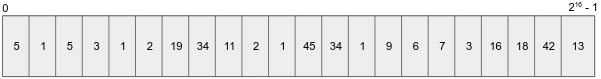
\includegraphics[width=0.7\textwidth]{rdbi-behavior-new}
    \caption{New procedure for scanning the RDBI service.}
    \label{fig:rdbi-behavior-new}
\end{figure}

The first point to answer is how the number of requests is calculated for each block. It is based on the probability of positive identifiers of this block. This probability is gathered from merging all positively answered identifiers of all ECUs and then for each block calculating $\frac{occurences}{block\_size}$. The number $r$ of requests for a block is calculated with
\[r(i, s)=\max(p(i, s) \cdot s, 1)\]
wherein $p$ stands for the probability function, $i$ for the index of the requested block and $s$ for the block size. For each block should be generated at least one request. The requested identifiers within a block are generated randomly.

The second question is which block size leads to the best results. This is again answered by a simulation. As potential block sizes $2^2, 2^3, ..., 2^{15}, 2^{16}$ were chosen because they are divisors for 2\textsuperscript{16}. The resulting coverages and request savings are then calculated for each ECU specifically and averaged to the final result. Same as for the RC service, the states are ignored in the simulation.

The approach has a feature which makes the simulation more complex than the former simulation. Since the blocks are first scanned randomly, the scan can lead to a great coverage, but also a low one, depending on the hit rate of the generated identifiers. To reduce this effect, the simulation is made 100 times, each time with newly created random identifiers. The 100 results are averaged to the coverage and request saving corrected from the random factor. This leads to a high processing time. To reduce the runtime, the execution was parallelized.
The following pseudocode shows the procedure more clearly.

\begin{samepage}
\begin{minted}{python}
for exponent in range(2, 16):
    block_size = 2 ** exponent
    coverages = []
    samples = []
    probabilities = get_probabilities(ecus, block_size)
    for ecu in ecus:
        for i in range(100):
            samples = random_samples(block_size, probabilities)
            positive_identifiers = ecu.get_positive_identifiers(samples)
            block_list = to_blocks(positive_identifiers, block_size)
            positive_identifiers = ecu.get_positive_identifiers(block_list)

            coverages.append(get_coverage(ecu, positive_identifiers))
            samples.append(len(block_list))
        avg_coverages, avg_samples = avg(coverages, samples)
\end{minted}
\end{samepage}

This simulation leads to \autoref{fig:rdbi-simulation-result}.

\begin{figure}[h]
    \centering
    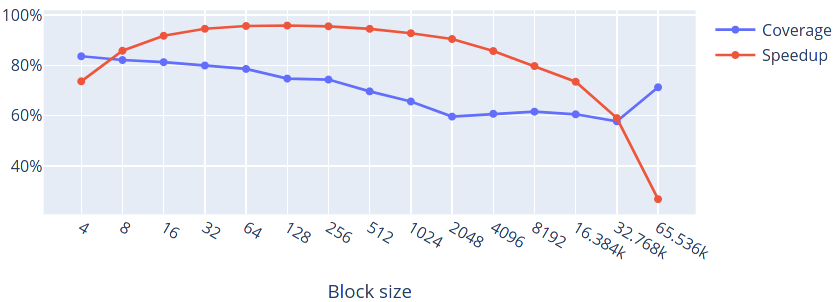
\includegraphics[width=0.8\textwidth]{rdbi-simulation-result}
    \caption{Simulation result for the RDBI service.}
    \label{fig:rdbi-simulation-result}
\end{figure}

The request saving is no longer linear; instead, it is highest for medium block sizes. From block sizes 64 to 128, the coverage decreases by 4\% while the request saving remains the same. Thus, it was decided for \textbf{64} as the block size leading to best results.


\subsection{Avoid the scan of unsupported services}
\label{subsec:unsupported-services-elaboration}

Each ECU usually supports only a subset of the services offered  by the UDS standard. This approach aims to avoid scanning them in order to save requests and therefore, time.

The first thing to understand is how to tell if a service is supported or not. The UDS standard defines the general server response behavior, shown in \autoref{fig:server-response-behaviour} with the important area highlighted.

\begin{figure}[h]
    \centering
    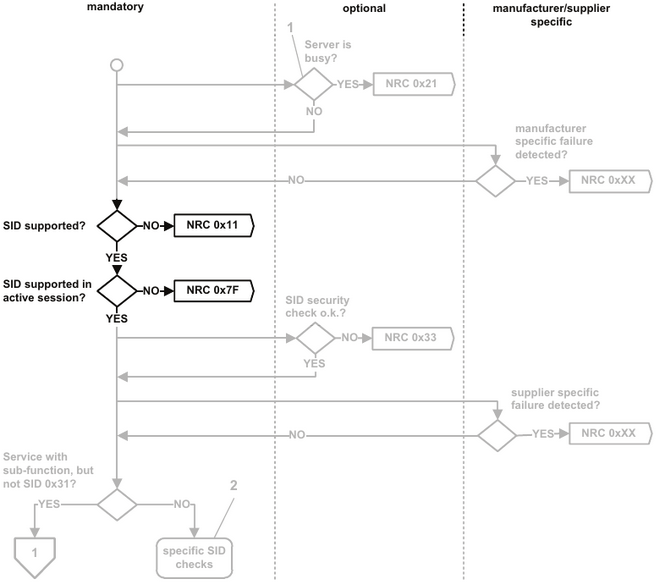
\includegraphics[width=0.8\textwidth]{server-response-behaviour}
    \caption{General server response behavior \cite{iso14229}. SID = service identifier.}
    \label{fig:server-response-behaviour}
\end{figure}

Each request is answered by a response, either positive or negative. A negative response contains a negative response code (NRC). \autoref{fig:server-response-behaviour} shows that the NRCs 0x11 and 0x7f are relevant for this approach. 0x11 indicates that the requested service is not supported at all. 0x7f is a lighter response code because it shows that the requested service is not supported in the current state of the ECU. Both response codes are sufficient to stop the current service scan with the current state and start with the next one. Although a 0x11 NRC is received, this service is still probed in other states. This is because with this behavior, in the worst case, one request is generated for this service for each state, which in turn receives 0x11 NRC again and then stops the service scan. The number of states detected is usually one-digit, so the number of packets generated is negligible. But in the best case the vendor has implemented the NRC incorrectly and the service is available in a different state.

\chapter{Implementation}

In this chapter, the theoretical explanations of the previous chapters are transferred into practical implementations with Python.

\section{Overview}

First, an overview is given to make the implementation easier to follow.

\subsection{Scapy modules for UDS scanning}

\begin{figure}[htb]
    \centering
    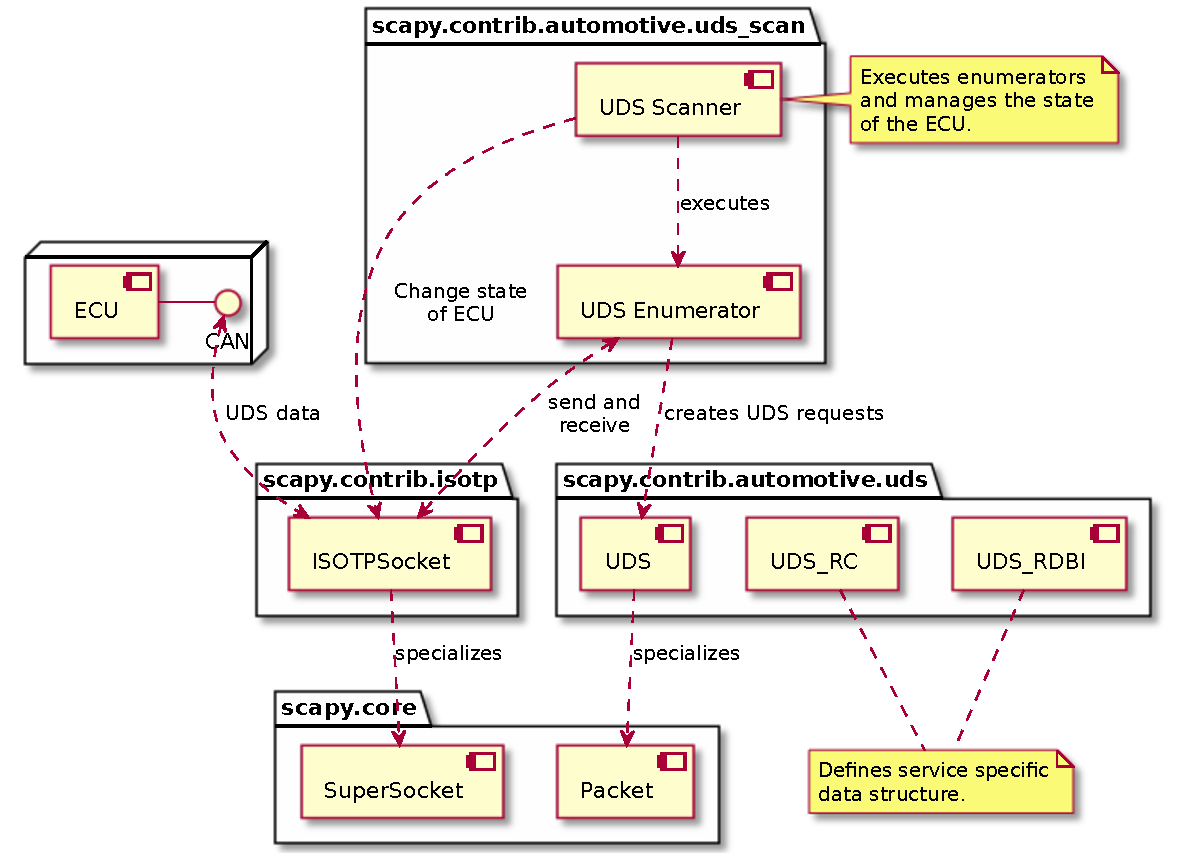
\includegraphics[width=0.83\textwidth]{uml/context}
    \caption{Interconnected modules of Scapy for UDS scanning.}
    \label{fig:uml-context}
\end{figure}

Scapy is a large program with many functions for all possible use cases. For a UDS scan, its modules shown in \autoref{fig:uml-context} are used together. Basically it needs four components:

\begin{itemize}
    \item An ISO-TP socket for communication with the ECU (see \autoref{subsec:isotp}).
    \item The UDS data structure definitions to generate requests and interpret responses (see \autoref{subsec:uds-scapy}).
    \item Service enumerators, which generate UDS requests. Only here changes were made.
    \item The UDS Scanner, which executes the enumerators and manages the state of the ECU.
\end{itemize}


\subsection{Service enumerators}

Enumerators are service-specific and create all possible requests for a service. For example, the enumerator of the RDBI service is called \mintinline{python}{UDS_RDBIEnumerator}. They are explained in more detail in \autoref{sec:enumerators}.

\begin{figure}[htb]
    \centering
    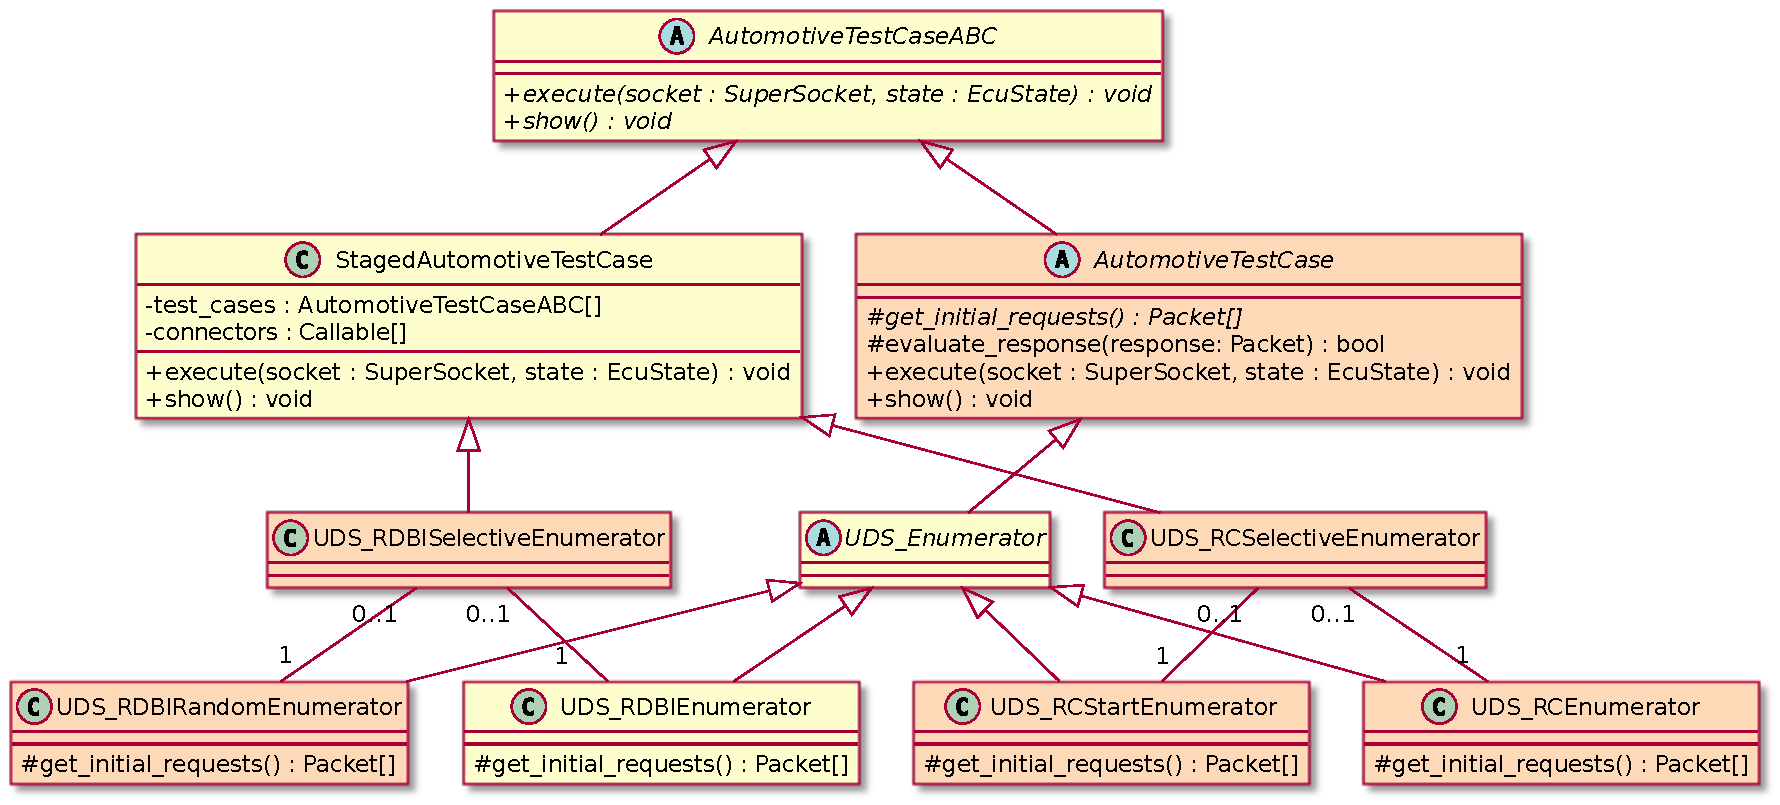
\includegraphics[width=1\textwidth]{uml/enumerators}
    \caption{Class diagram of some enumerators.}
    \label{fig:uml-enumerators}
\end{figure}

\autoref{fig:uml-enumerators} shows the class tree of some enumerators and their super classes. The classes with a darker background are the classes that were modified or created for this thesis. The root is the \mintinline{python}{AutomotiveTestCaseABC} class. It requires each subclass to implement the \mintinline{python}{execute} method. Its first parameter \mintinline{python}{socket} specifies on which socket the requests and responses are communicated. \mintinline{python}{SuperSocket} is the root class of Scapy for all sockets. For the UDS Scanner, this is usually an \mintinline{python}{ISOTPSocket}.

In general, a scanner like the UDS Scanner executes automotive test cases. For a normal UDS scan, these test cases are only service enumerators. However, other test cases are also conceivable. The inheritance tree of all enumerators starts at \mintinline{python}{AutomotiveTestCaseABC}. This is the type that is expected from scanners.
Staged enumerators inherit from \mintinline{python}{StagedAutomotiveTestCase} and single enumerators from \mintinline{python}{AutomotiveTestCase}. The \mintinline{python}{UDS_Enumerator} defines UDS-specific behavior that it doesn't need to be specified again for each UDS enumerator. For example, how the negative response code (NRC) of a response is read.

The most important member of the enumerator classes is the \mintinline{python}{get_initial_requests} method. The return value is an iterable object which contains the requests for this service. It actually has a parameter which enables the caller to configure the enumerator. Due to lack of space it is hidden in \autoref{fig:uml-enumerators}. The full diagram can be seen in \autoref{app:uml}.


\subsection{Scanner classes}

\begin{figure}[htb]
    \centering
    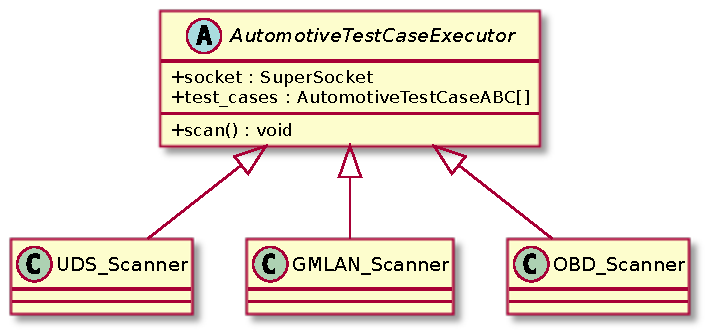
\includegraphics[width=0.6\textwidth]{uml/scanners}
    \caption{Class diagram of the protocol scanners.}
    \label{fig:uml-scanners}
\end{figure}

\autoref{fig:uml-scanners} shows the class diagram of the three protocol scanners in Scapy. Each is given a list of test cases (see \autoref{fig:uml-enumerators}) and a socket that is passed to each test case's \mintinline{python}{execute} method. Their \mintinline{python}{scan} method starts a scan.

\subsection{Dependencies}

First, a Python interpreter is required.
The enumerators and the UDS Scanner itself are implemented in Scapy. Therefore, Scapy must also be installed. The last dependency results from the socket used. If the native ISO-TP Socket is used, a Linux-based operating system is required and possibly the installation of a driver module (see \autoref{subsec:isotp}). For using a CAN bus without Linux the 'python-can' library is needed. Complete instructions can be found in the Scapy documentation. For a scan over an Ethernet interface, no further action is necessary.

\subsection{Usage}

A minimal example that uses the new enumerators and skips unsupported services can be run as shown in \autoref{lst:usage}. All implementations of the approaches are used with this code. The \mintinline{python}{UDS_RCSelectiveEnumerator} (approach 1), the \mintinline{python}{UDS_RDBISelectiveEnumerator} (approach 2) and \mintinline{python}{exit_if_service_not_supported} (approach 3). Since this is a minimal example and neither the RC nor the RDBI service change the state of the ECU, this scan would not detect any other states besides the default state. To detect further states, the \mintinline{python}{UDS_DSCEnumerator} should be included.



\begin{listing}[H]
\begin{minted}
[frame=single,
framerule=0pt,
framesep=2mm,
baselinestretch=1.2,
bgcolor=VeryLightGray,
fontsize=\footnotesize,
linenos]
{python}
with ISOTPSocket("can0", sid=0x6fd, did=0x610, basecls=UDS) as tester:
    enumerators = [UDS_RCSelectiveEnumerator, UDS_RDBISelectiveEnumerator]
    scanner = UDS_Scanner(tester, test_cases=es, exit_if_service_not_supported=True)
    scanner.scan()

\end{minted}
\caption{Using the UDS Scanner with the new enumerators and behavior.}
\label{lst:usage}
\end{listing}

\section{Explaining the service enumerators of the UDS Scanner}
\label{sec:enumerators}

Enumerators are service-specific and generate UDS requests for a service.
Each enumerator will be executed for each found state of the ECU. So, if an enumerator already was executed, and afterwards a new state is found by the UDS Scanner, this enumerator will be executed again within the same scan with the new-found state.

For a better understanding, the \mintinline{python}{UDS_DSCEnumerator} implementation for the DSC service will be described exemplary.

\begin{listing}[H]
\begin{minted}
[frame=single,
framerule=0pt,
framesep=2mm,
baselinestretch=1.2,
bgcolor=VeryLightGray,
fontsize=\footnotesize,
linenos]
{python}
class UDS_DSCEnumerator(UDS_Enumerator, StateGenerator):
    def _get_initial_requests(self, **kwargs):
        session_range = kwargs.pop('session_range', range(2, 0x100))
        return UDS() / UDS_DSC(diagnosticSessionType=session_range)
\end{minted}
\caption{Implementation of the enumerator scanning the DSC service.}
\label{lst:dsc-enumerator}
\end{listing}

Its \mintinline{python}{get_initial_requests} method can be configured by keyword parameters. The only one read by this method implementation is \mintinline{python}{session_range}. If none is given, which is usually the case, it defaults to the range from \mintinline{text}{0x02} to \mintinline{text}{0xff}. So, this enumerator creates 254 requests for each state by default. It is also a \mintinline{python}{StateGenerator}, which means its requests can change the state of the ECU (see \autoref{subsec:states}). This is detected by the UDS Scanner and the new state will be scanned as well.

Enumerators can output their results as a text-table. For example a possible output of the UDS enumerator is:

\begin{samepage}
\begin{minted}[fontsize=\footnotesize]{text}
----------+--------------------------+--------------------------+--------------------------+
          | defaultState             | state2                   | state3                   | 
----------+--------------------------+--------------------------+--------------------------+
0x02      | PR: Supported            | NR: -                    | NR: -                    | 
0x03      | NR: -                    | PR: Supported            | NR: -                    | 
0x82      | NR: conditionsNotCorrect | NR: -                    | NR: -                    | 
----------+--------------------------+--------------------------+--------------------------+
\end{minted}
\end{samepage}

Each row is a request. Here are listed requests of the DSC service with parameters \mintinline{text}{0x02}, \mintinline{text}{0x03} and \mintinline{text}{0x82}. Each column is a state. And each cell shows the response for each request per state (PR = positive response, NR = negative response).

A PenTester is able to extract a state machine from this table (see \autoref{fig:state-machine-of-scan}).

\begin{figure}[H]
    \centering
    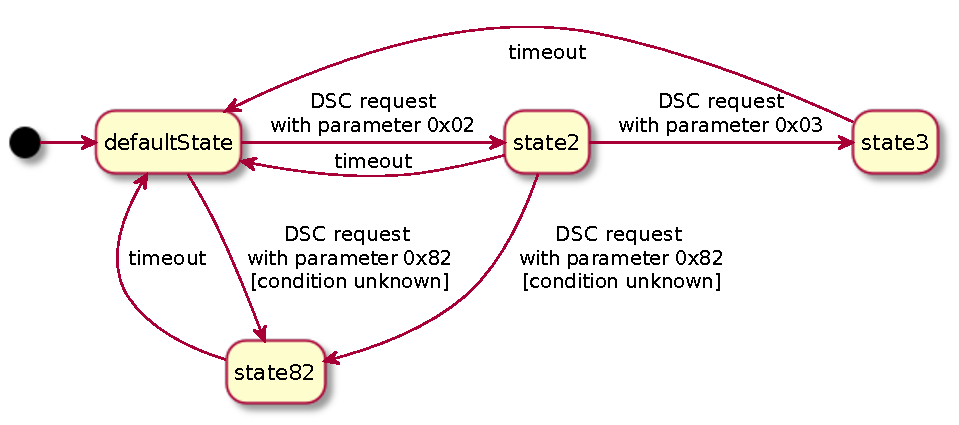
\includegraphics[width=0.7\textwidth]{uml/dsc-state-machine}
    \caption{Partial result for a PenTester of a UDS scan.}
    \label{fig:state-machine-of-scan}
\end{figure}

So-called staged enumerators contain enumerators where each enumerator is a stage. They start executing the first enumerator for each state, followed by each subsequent enumerator in the same way (see \autoref{fig:uml-staged-enumerators}).


\begin{figure}[htb]
    \centering
    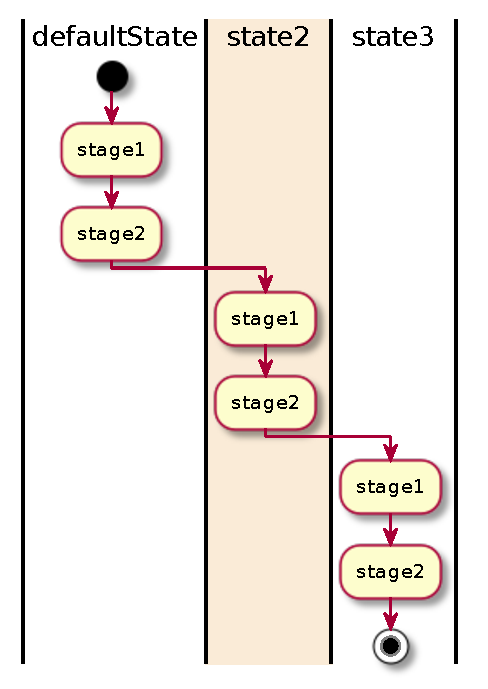
\includegraphics[width=0.35\textwidth]{uml/staged-enumerators}
    \caption{The sequence of a two-staged enumerator.}
    \label{fig:uml-staged-enumerators}
\end{figure}

For each stage transition connectors can be defined. They are functions with two arguments, containing the previous enumerator and the new enumerator. Here, the results of the previous enumerator can be evaluated and the next enumerator can be configured accordingly. The connector will be automatically called by the UDS Scanner and expects a dictionary as return value that will be passed to the next enumerator. In \autoref{fig:uml-staged-enumerators}, each arrow represents a call of a connector, except for the first and last arrows. \autoref{lst:staged-enumerator} shows a simple definition of a staged enumerator.

\begin{listing}[H]
\begin{minted}
[frame=single,
framerule=0pt,
framesep=2mm,
baselinestretch=1.2,
bgcolor=VeryLightGray,
fontsize=\footnotesize,
linenos]
{python}
class MyStagedEnumerator(StagedAutomotiveTestCase):
    @staticmethod
    def connector_stage1_stage2(stage1_enum, stage2_enum):
        results = stage1_enum.get_results()
        stage2_config = create_config(results)
        return stage2_config
    
    def __init__(self):
        super().__init__(
            [Stage1Enumerator(), Stage2Enumerator()],
            connectors=[None, self.connector_stage1_stage2])
\end{minted}
\caption{Example implementation of a staged enumerator.}
\label{lst:staged-enumerator}
\end{listing}

\section{Implementing enumerators for the RC service}

Three classes are of interest:

\begin{itemize}
    \item \mintinline{python}{RCEnumerator}: Defaults to scanning the whole RC service, including all three types.
    \item \mintinline{python}{RCStartEnumerator}: Only scanning type1 of the RC service.
    \item \mintinline{python}{RCSelectiveEnumerator}: Staged enumerator containing an RCStartEnumerator and an RCEnumerator.
\end{itemize}

For this work, the configurability of the \mintinline{python}{RCEnumerator} was improved, and the \mintinline{python}{RCStartEnumerator} and \mintinline{python}{RCSelectiveEnumerator} were created. \autoref{fig:rc-schematic} provides an initial overview of the new implementation mechanisms.

\begin{figure}[htb]
    \centering
    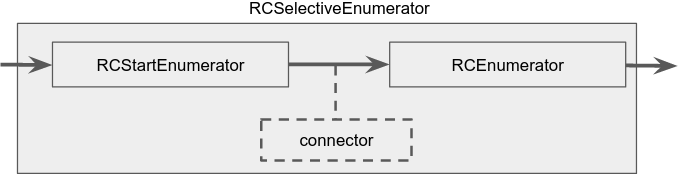
\includegraphics[width=0.7\textwidth]{rc-schematic}
    \caption{Schematic illustration of the new \mintinline{python}{RCSelectiveEnumerator}.}
    \label{fig:rc-schematic}
\end{figure}

First, the \mintinline{python}{RCEnumerator} will be explained by having a closer look at its \mintinline{python}{get_initial_requests} method.

\begin{listing}[H]
\begin{minted}
[frame=single,
framerule=0pt,
framesep=2mm,
baselinestretch=1.2,
bgcolor=VeryLightGray,
fontsize=\footnotesize,
linenos]
{python}
class UDS_RCEnumerator(UDS_Enumerator):
    def _get_initial_requests(self, **kwargs):
        type_list = kwargs.pop("type_list", [1, 2, 3])
        scan_range = kwargs.pop("scan_range", range(0x10000))

        return (
            UDS() / UDS_RC(routineControlType=rc_type,
                           routineIdentifier=data_id)
            for rc_type, data_id in itertools.product(type_list, scan_range)
        )
\end{minted}
\caption{The extended enumerator for the RC service.}
\label{lst:rc-enumerator}
\end{listing}

Two parameters can be configured, the \mintinline{python}{type_list} and \mintinline{python}{scan_range}. Both default to the values required to scan the whole RC service. Eventually, the method returns a generator that generates all requests possible by pairing the values of \mintinline{python}{type_list} and \mintinline{python}{scan_range}. This accomplishes the \mintinline{python}{itertools.product} method from the Python Standard library. It returns the cartesian product of the input iterables.

Next, the \mintinline{python}{RCStartEnumerator}.

\begin{listing}[H]
\begin{minted}
[frame=single,
framerule=0pt,
framesep=2mm,
baselinestretch=1.2,
bgcolor=VeryLightGray,
fontsize=\footnotesize,
linenos]
{python}
class UDS_RCStartEnumerator(UDS_RCEnumerator):
    def _get_initial_requests(self, **kwargs):
        kwargs["type_list"] = [1]
        return super()._get_initial_requests(**kwargs)
\end{minted}
\caption{The enumerator for the RC service scanning only type1.}
\label{lst:rc-start-enumerator}
\end{listing}

Its \mintinline{python}{get_initial_requests} method is simple. It fixes the \mintinline{python}{type_list} to type1 and then calls its implementation of the super class, which is the previously explained \mintinline{python}{UDS_RCEnumerator}. This results in generating requests only for type1.

The \mintinline{python}{UDS_RCSelectiveEnumerator} connects both of these enumerators.

\begin{listing}[H]
\begin{minted}
[frame=single,
framerule=0pt,
framesep=2mm,
baselinestretch=1.2,
bgcolor=VeryLightGray,
fontsize=\footnotesize,
linenos]
{python}
class UDS_RCSelectiveEnumerator(StagedAutomotiveTestCase):
    expansion_width = 253

    @staticmethod
    def connector_start_to_full(rc_start, rc_full):
        identifiers_with_pr = [r.resp.routineIdentifier for r
                            in rc_start.results_with_positive_response]

        scan_range = points_to_ranges(
            identifiers_with_pr, UDS_RCSelectiveEnumerator.expansion_width)

        return {"type_list": [2, 3],
                "scan_range": scan_range}

    def __init__(self):
        super().__init__(
            [UDS_RCStartEnumerator(), UDS_RCEnumerator()],
            [None, self.connector_start_to_full])
\end{minted}
\caption{The staged enumerator combining the start and complete enumerator for the RC service.}
\label{lst:rc-selective-enumerator}
\end{listing}

This staged enumerator has the \mintinline{python}{RCStartEnumerator} as the first stage, and the \mintinline{python}{RCEnumerator} as the second and last stage.
The expansion width is fixed to \textbf{253} as it was elaborated in \autoref{subsubsec:rc-elaborating}.

The connector calls \mintinline{python}{points_to_ranges} to expand the found identifiers of the first stage to ranges and passes them to the second stage. In addition, the connector configures the \mintinline{python}{RCEnumerator} to scan only type2 and type3, since type1 should no longer be scanned.

\begin{listing}[H]
\begin{minted}
[frame=single,
framerule=0pt,
framesep=2mm,
baselinestretch=1.2,
bgcolor=VeryLightGray,
fontsize=\footnotesize,
linenos]
{python}
def points_to_ranges(points, expansion_width):
    generators = []
    for identifier in points:
        start = max(identifier - expansion_width, 0)
        end = min(identifier + expansion_width + 1, 0x10000)
        generators.append(range(start, end))
    ranges_with_overlaps = itertools.chain.from_iterable(generators)
    return sorted(set(ranges_with_overlaps))
\end{minted}
\caption{Function extending points to ranges.}
\label{lst:points-to-ranges}
\end{listing}

\mintinline{python}{points_to_ranges} expands points to ranges and also resolves any overlaps to a continuous range.
First, a range generator is created for each given point. Then, they are chained and converted to a set, removing potential overlaps. This set is sorted in a list, to ensure understandable candump logs of a scan.

\section{Implementing enumerators for the RDBI service}

Again, three classes are of interest:

\begin{itemize}
    \item \mintinline{python}{RDBIEnumerator}: Defaults to scanning the whole RDBI service.
    \item \mintinline{python}{RDBIRandomEnumerator}: Scanning block-based with random identifiers.
    \item \mintinline{python}{RDBISelectiveEnumerator}: Staged enumerator containing an RDBIRandomEnumerator and an RDBIEnumerator.
\end{itemize}

The new implementation is two-staged. First, the \mintinline{python}{RDBIRandomEnumerator} is executed. Then, the connector creates requests for whole blocks, if any of their requests were answered positively, and ensured that for a single block each identifier is queried only once. The resulting requests are passed to the configurable \mintinline{python}{RDBIEnumerator}. \autoref{fig:rdbi-schematic} shows that schematically.

\begin{figure}[htb]
    \centering
    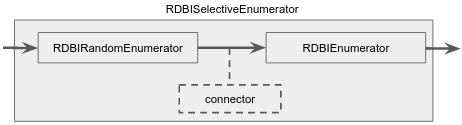
\includegraphics[width=0.7\textwidth]{rdbi-schematic}
    \caption{Schematic illustration of the new \mintinline{python}{RDBISelectiveEnumerator}.}
    \label{fig:rdbi-schematic}
\end{figure}

The explanation starts with the original enumerator, here the \mintinline{python}{RDBIEnumerator}.

\begin{listing}[H]
\begin{minted}
[frame=single,
framerule=0pt,
framesep=2mm,
baselinestretch=1.2,
bgcolor=VeryLightGray,
fontsize=\footnotesize,
linenos]
{python}
class UDS_RDBIEnumerator(UDS_Enumerator):
    def _get_initial_requests(self, **kwargs):
        scan_range = kwargs.pop("scan_range", range(0x10000))
        return (UDS() / UDS_RDBI(identifiers=[x]) for x in scan_range)
\end{minted}
\caption{The enumerator scanning the whole RDBI service by default.}
\label{lst:rdbi-enumerator}
\end{listing}

Since the RDBI service has only one parameter, its \mintinline{python}{get_initial_requests} remains simple, generating RDBI requests for identifiers from 0 to 65,535, if not configured otherwise.

Implementing the \mintinline{python}{RDBIRandomEnumerator} was a challenge because it must include the count of requests for each block. With a block size of \textbf{64} (see \autoref{subsubsec:rdbi-behavior}), there would need to be a list with $\frac{2^{16}}{64} = 1024$ elements. Thus, it is desirable to represent this information more compactly. A better representation is based on the fact that many blocks have a calculated number of requests of zero, but at least one request should be generated for each block. So, the number of samples is not stored for all blocks, but only for blocks whose number of samples is greater than or equal to two. And for blocks for which no value is stored, the value one is derived. This automatically solves that each block is probed with at least one request. These simplifications transformed the list of 1024 elements into a dictionary of only 109 elements. The non-simplified version is shown in \autoref{app:random-not-compact}.

\begin{listing}[H]
\begin{minted}
[frame=single,
framerule=0pt,
framesep=2mm,
baselinestretch=1.2,
bgcolor=VeryLightGray,
fontsize=\footnotesize,
linenos]
{python}
class UDS_RDBIRandomEnumerator(UDS_RDBIEnumerator):
    def _get_initial_requests(self, **kwargs):
        samples_per_block = {
            4: 29, 5: 22, 6: 19, 8: 11, 9: 11, 10: 13, 11: 14,
            # [...]
            1013: 14, 1014: 15
        }
        to_scan = []
        block_size = UDS_RDBIRandomEnumerator.block_size
        for block_index, start in enumerate(range(0, 2 ** 16, block_size)):
            end = start + block_size
            count_samples = samples_per_block.get(block_index, 1)
            to_scan += random.sample(range(start, end), count_samples)

        positive_identifiers = [t.resp.dataIdentifier for t in
                                self.results_with_positive_response]
        to_scan += positive_identifiers

        to_scan = sorted(list(set(to_scan)))
        return (UDS() / UDS_RDBI(identifiers=[x]) for x in to_scan)
\end{minted}
\caption{The enumerator scanning randomly the RDBI service based on blocks.}
\label{lst:rdbi-random-enumerator}
\end{listing}

The \mintinline{python}{random.sample} function from the Python Standard library returns a list of given length with unique elements chosen from the given sequence.

The implementation exploits the observation that most identifiers are available in multiple states. Thus, the randomly generated identifiers are appended with the identifiers that were answered positively in any previous state.

Again, the \mintinline{python}{UDS_RDBISelectiveEnumerator} brings these two enumerators together.

\begin{listing}[H]
\begin{minted}
[frame=single,
framerule=0pt,
framesep=2mm,
baselinestretch=1.2,
bgcolor=VeryLightGray,
fontsize=\footnotesize,
linenos]
{python}
class UDS_RDBISelectiveEnumerator(StagedAutomotiveTestCase):
    block_size = 2 ** 6

    @staticmethod
    def connector_random_to_sequential(rdbi_random, rdbi_full):
        identifiers_with_pr = \
            [r.resp.dataIdentifier
            for r in rdbi_random.results_with_positive_response]

        scan_range = points_to_blocks(
                identifiers_with_pr,
                UDS_RDBISelectiveEnumerator.block_size)
        return {"scan_range": scan_range}

    def __init__(self):
        super().__init__(
            [UDS_RDBIRandomEnumerator(), UDS_RDBIEnumerator()],
            [None, self.connector_random_to_sequential])
\end{minted}
\caption{The staged enumerator combining the random and complete enumerator for the RDBI service.}
\label{lst:rdbi-selective-enumerator}
\end{listing}

Since it is similar to the \mintinline{python}{RCSelectiveEnumerator}, it will not be explained any further. Only the \mintinline{python}{points_to_blocks} will be described in more detail.

\begin{listing}[H]
\begin{minted}
[frame=single,
framerule=0pt,
framesep=2mm,
baselinestretch=1.2,
bgcolor=VeryLightGray,
fontsize=\footnotesize,
linenos]
{python}
def points_to_blocks(points, block_size):
    generators = []
    for start in range(0, 2 ** 16, block_size):
        end = start + block_size
        pr_in_block = any((start <= identifier < end
                        for identifier in points))
        if pr_in_block:
            generators.append(range(start, end))
    scan_range = itertools.chain.from_iterable(generators)
    return scan_range
\end{minted}
\caption{Function extending points to fixed blocks.}
\label{lst:points-to-blocks}
\end{listing}

Unlike \mintinline{python}{points_to_ranges}, its block boundaries are fixed. It traverses each block and checks if any of the given identifiers is part of that block. If this is the case, the block will be scanned completely.

Unfortunately, this can lead to double-scanned identifiers, since instead of scanning only the remaining identifiers that have not yet been scanned in the respective blocks, the entire blocks are rescanned. Although an attempt was made to implement this, the UDS scanner does not provide the necessary interfaces to do so. The connectors only know the enumerators, but not the currently executed state. However, this is necessary to check which identifiers have already been scanned in the random enumerator for the current state. Nevertheless, the number of duplicate requests is low, so the request savings hardly decrease.

\section{Extending the enumerators to skip unsupported services}

In contrast to the previous approaches, this one is not applied to specific service enumerators, but to their super class. It evaluates each response, for example to detect if a new state was found. Here, a check was added for negative responses if they have an NRC of \mintinline{text}{0x11} or \mintinline{text}{0x7f}. If they do, the enumerator is set to completed for the currently executed state.

\begin{listing}[H]
\begin{minted}
[frame=single,
framerule=0pt,
framesep=2mm,
frame=single,
framerule=0pt,
framesep=2mm,
baselinestretch=1.2,
bgcolor=VeryLightGray,
fontsize=\footnotesize,
linenos]
{python}
class AutomotiveTestCase(AutomotiveTestCaseABC):
    """Base class for Enumerators"""

    def _evaluate_response(self, response, **kwargs):

        # Removed code for simplification

        if exit_if_service_not_supported and response.service == 0x7f:
            response_code = self._get_negative_response_code(response)
            if response_code in [0x11, 0x7f]:
                # execute of current state is completed,
                # since a serviceNotSupported NR was received
                current_state = self._results[-1].state
                self._state_completed[current_state] = True
                # stop current execute and exit
                return True

        # Removed code for simplification

        return False
\end{minted}
\caption{The extended super class of each enumerator with skipping unsupported services.}
\label{lst:enumerator-super-class}
\end{listing}    

\chapter{Results on ECUs}

This section shows and discusses the results of the implementations explained earlier.

\section{Coverages and request savings}

First, the coverages and request savings are assessed for each approach.

\subsection{Reusing information within the same service}

\begin{table}[H]
    \begin{center}
    \begin{tabular}{ccc}
        \hline
        & \textbf{Coverage} & \textbf{Request saving} \\
        \hline
        \textbf{audi\_cgw} & 87.6\% & 65.4\% \\
        \textbf{bfft-ecu} & 100\% & 66.2\% \\
        \textbf{bmw-gateway-ecu-bdc} & 100\% & 66.2\% \\
        \textbf{bmw-gateway-ecu-zgw} & 100\% & 64.5\% \\
        \textbf{bmw-gateway-ecu2} & 100\% & 64.6\% \\
        \textbf{bmw-tcu} & 100\% & 66.7\% \\
        \textbf{bosch-ecu} & 100\% & 64.6\% \\
        \textbf{dashboard} & 50.0\% & 66.2\% \\
        \textbf{mercedes-ezs} & 100\% & 65.1\% \\
        \textbf{seppmed} & 100\% & 66.2\% \\
        \textbf{tesla-airbag-ecu} & 100\% & 66.7\% \\
        \hline

    \end{tabular}
    \end{center}
    \caption{Measured coverages and request savings on ECUs with approach 1 for the RC service.}
    \label{tab:evaluation-approach1}
\end{table}

9 of 11 ECUs had a full coverage. The coverage for the dashboard ECU is notable low. Therefore, a closer look was taken there. It turned out that the Dashboard only supports two identifiers. The identifier 515 for Type1 and identifier 61,728 for Type3. The former is detected, but the resulting range for Type3 is far from the identifier 61,728. Hence, the loss and a coverage of 50\%.

For each ECU the request saving is close to the theoretical maximum of $66.7$ \%. It is so high because ECUs usually support only a few routines (see \autoref{fig:rc-distribution}). Hence, only a few identifiers are expanded to blocks and lead to more requests.

This approach is applicable to scans of services with multiple parameters. This results in a high scan time for this service and thus a high time-saving potential. However, if an identifier is not recognized during the first scan, it will not be recognized in the next scans as well.


\subsection{Using probabilities of positive answers based on blocks}

\begin{table}[H]
    \begin{center}
    \begin{tabular}{ccc}
        \hline
        & \textbf{Coverage} & \textbf{Request saving} \\
        \hline
        \textbf{audi\_cgw} & 87.8\% & 85.0\% \\
        \textbf{bfft-ecu} & 88.4\% & 96.6\% \\
        \textbf{bmw-gateway-ecu-bdc} & 100\% & 96.1\% \\
        \textbf{bmw-gateway-ecu-zgw} & 94.3\% & 95.8\% \\
        \textbf{bmw-gateway-ecu2} & 83.3\% & 96.1\% \\
        \textbf{bmw-tcu} & 72.2\% & 96.3\% \\
        \textbf{bosch-ecu} & 90.7\% & 93.3\% \\
        \textbf{dashboard} & 92.4\% & 94.4\% \\
        \textbf{mercedes-ezs} & 89.3\% & 94.7\% \\
        \textbf{seppmed} & 83.0\% & 95.9\% \\
        \textbf{tesla-airbag-ecu} & 100\% & 96.4\% \\
        \hline
    \end{tabular}
    \end{center}
    \caption{Measured coverages and request savings on ECUs with approach 2 for the RDBI service.}
    \label{tab:evaluation-approach2}
\end{table}

\autoref{tab:evaluation-approach2} shows the resulting coverage and request savings for this approach for the RDBI service. It should be noted, that these values vary slightly for each run because a random scan is used.

Overall, the coverages are lower with this approach than for approach 1. Only for two ECUs a coverage of 100\% is reached. The request savings are high at approximately 95\%. Nevertheless, the time savings of approach 1 are higher in practice, because that approach can be applied to larger service scans, and then a saving of about 66\% saves more time there than 95\% here.

The biggest problem with this approach is the newly added random factor. The coverage can be great for one scan, but low for the next one. This would require performing multiple scans using the new implementation to ensure that most identifiers were found.

\subsection{Not scanning unsupported services}

\autoref{fig:serviceNotSupported-savings} illustrates the number of saved packets for each ECU with this approach. It is only an approximation because for this graph, the responses with the both described NRCs (0x11 and 0x7f) have been counted. But actually, not every request can be saved with this approach, since at least one request must first be made to detect that this service is not supported. But this number of requests is low and negligible, especially considering that the minimum value of saved requests is about 70,000.

\begin{figure}[h]
    \centering
    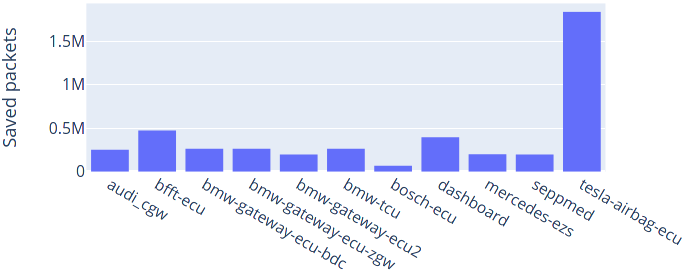
\includegraphics[width=0.8\textwidth]{serviceNotSupported-savings}
    \caption{Saved number of requests with this approach (approx).}
    \label{fig:serviceNotSupported-savings}
\end{figure}

There is a potential problem with this approach. Reliance is placed on the manufacturer to properly implement these NRCs. It is conceivable that the ECU responds to an identifier with 0x11 or 0x7f, although a subsequent identifier would actually have been answered positively. The occurrences of this behavior are shown in \autoref{fig:serviceNotSupported-losses}. It was calculated by evaluating the responses for each enumerator for each state. Once a negative response with NRC 0x11 or 0x7f was received, an internal counter was incremented with each subsequent positive response.
And in comparison to the potential savings (\autoref{fig:serviceNotSupported-savings}), the losses are negligible.

\begin{figure}[h]
    \centering
    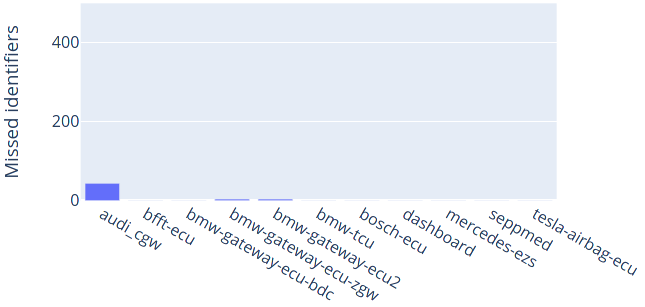
\includegraphics[width=0.8\textwidth]{serviceNotSupported-losses}
    \caption{Lost number of positive responses with this approach.}
    \label{fig:serviceNotSupported-losses}
\end{figure}

Skipping unsupported services is the safest way to save time of all three approaches. It is unlikely that identifiers will be missed, but the speed gain can still be high. Nevertheless, the option remains optional in the UDS scanner.

\section{Actual time savings}

For each ECU, the same scans were executed again as in the introduction (\autoref{sec:introduction}), they differ only in the use of the new implementations.

\begin{figure}[h]
    \centering
    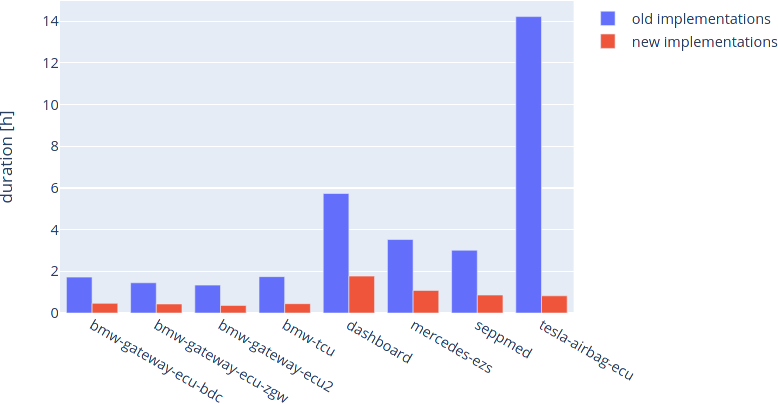
\includegraphics[width=1\textwidth]{durations-diff}
    \caption{Side by side illustration of runtimes of a UDS scan with old and new implementations.}
    \label{fig:durations-diff}
\end{figure}

As \autoref{fig:durations-diff} shows, the durations decreased significantly, especially for the Tesla ECU, which has a relatively high average response time (about 20 ms) compared to the others (1 – 8 ms).
Three ECUs are excluded from this observation because they were no longer available at the time of re-evaluating the scan durations.

\section{Conclusion and Future Work}

\subsection{Conclusion}

In this thesis, three approaches were evaluated to improve the efficiency of a UDS scan. The use of information within the same scan (approach 1), reducing the scan range (approach 2) and avoiding scanning unsupported services (approach 3).

All three approaches turned out to maintain a high speed-up while still offering a high coverage.
Nevertheless, all three approaches are not able to provide a 100\% coverage at all times. 
If a coverage of 100\% is desired, a full scan might be the preferred solution, even if it takes much longer. This may be acceptable, if this scan will be executed only once. For fast results and good, but possibly not complete coverage, the new implementation should be preferred. It depends on the use case. Therefore, the new enumerators are not a replacement for the original ones, but an addition.

\subsection{Future Work}

Reducing the scan range could also be applied to the IOCBI service. Theoretically, to many more services, but most of them only have 8-bit identifiers, leading to almost no time savings, thus not worth lower coverages.

Also, another approach can be evaluated. While elaborating this work, it was observed that manufacturers tend to use the same identifiers across their ECUs for the RDBI service. So, these identifiers could be collected, grouped by manufacturers and used for more precise scanning through fixing some requests accordingly instead of only scanning randomly. One could go one step further here and not only group by manufacturers, but also by ECU type.
For example, all available BMW ECUs turned out to have 11 identifiers in common. On the other site, the both available BMW central gateway ECUs turned out to have 61 identifiers in common. But for this approach, more data is necessary. For this work were ten unique ECUs available, which support UDS, wherein only from BMW more than one ECU was available. This is the reason why this approach was not pursued further.
For example, it turned out that all available BMW ECUs have 11 identifiers in common. On the other hand, it turned out that the two available BMW Central Gateway ECUs have 61 identifiers in common. However, more data is needed for this approach. For this work, ten unique ECUs supporting UDS were available, with only BMW having more than one available. This is the reason why this approach was not pursued.

Approach 1 and approach 2 could be merged. For example, Type1 of the RC service is no longer scanned completely, but randomly based on probabilities. Unchanged is the second stage, where Type2 and Type3 are scanned based on the results of the first stage. This probably leads to even higher speed increases, but also to lower coverages.

In addition, the UDS Scanner and enumerators are not yet part of the official Scapy repository at press time. They will be refined and gradually added to the official repository.


\include{chapters/8_closing-words}

\thispagestyle{plain}
\printunsrtglossary[type=\acronymtype]

\thispagestyle{plain}
\listoffigures

\thispagestyle{plain}
\printbibliography

\chapter{Class diagram of enumerator classes}
\label{app:uml}

\begin{figure}[H]
    \centering
    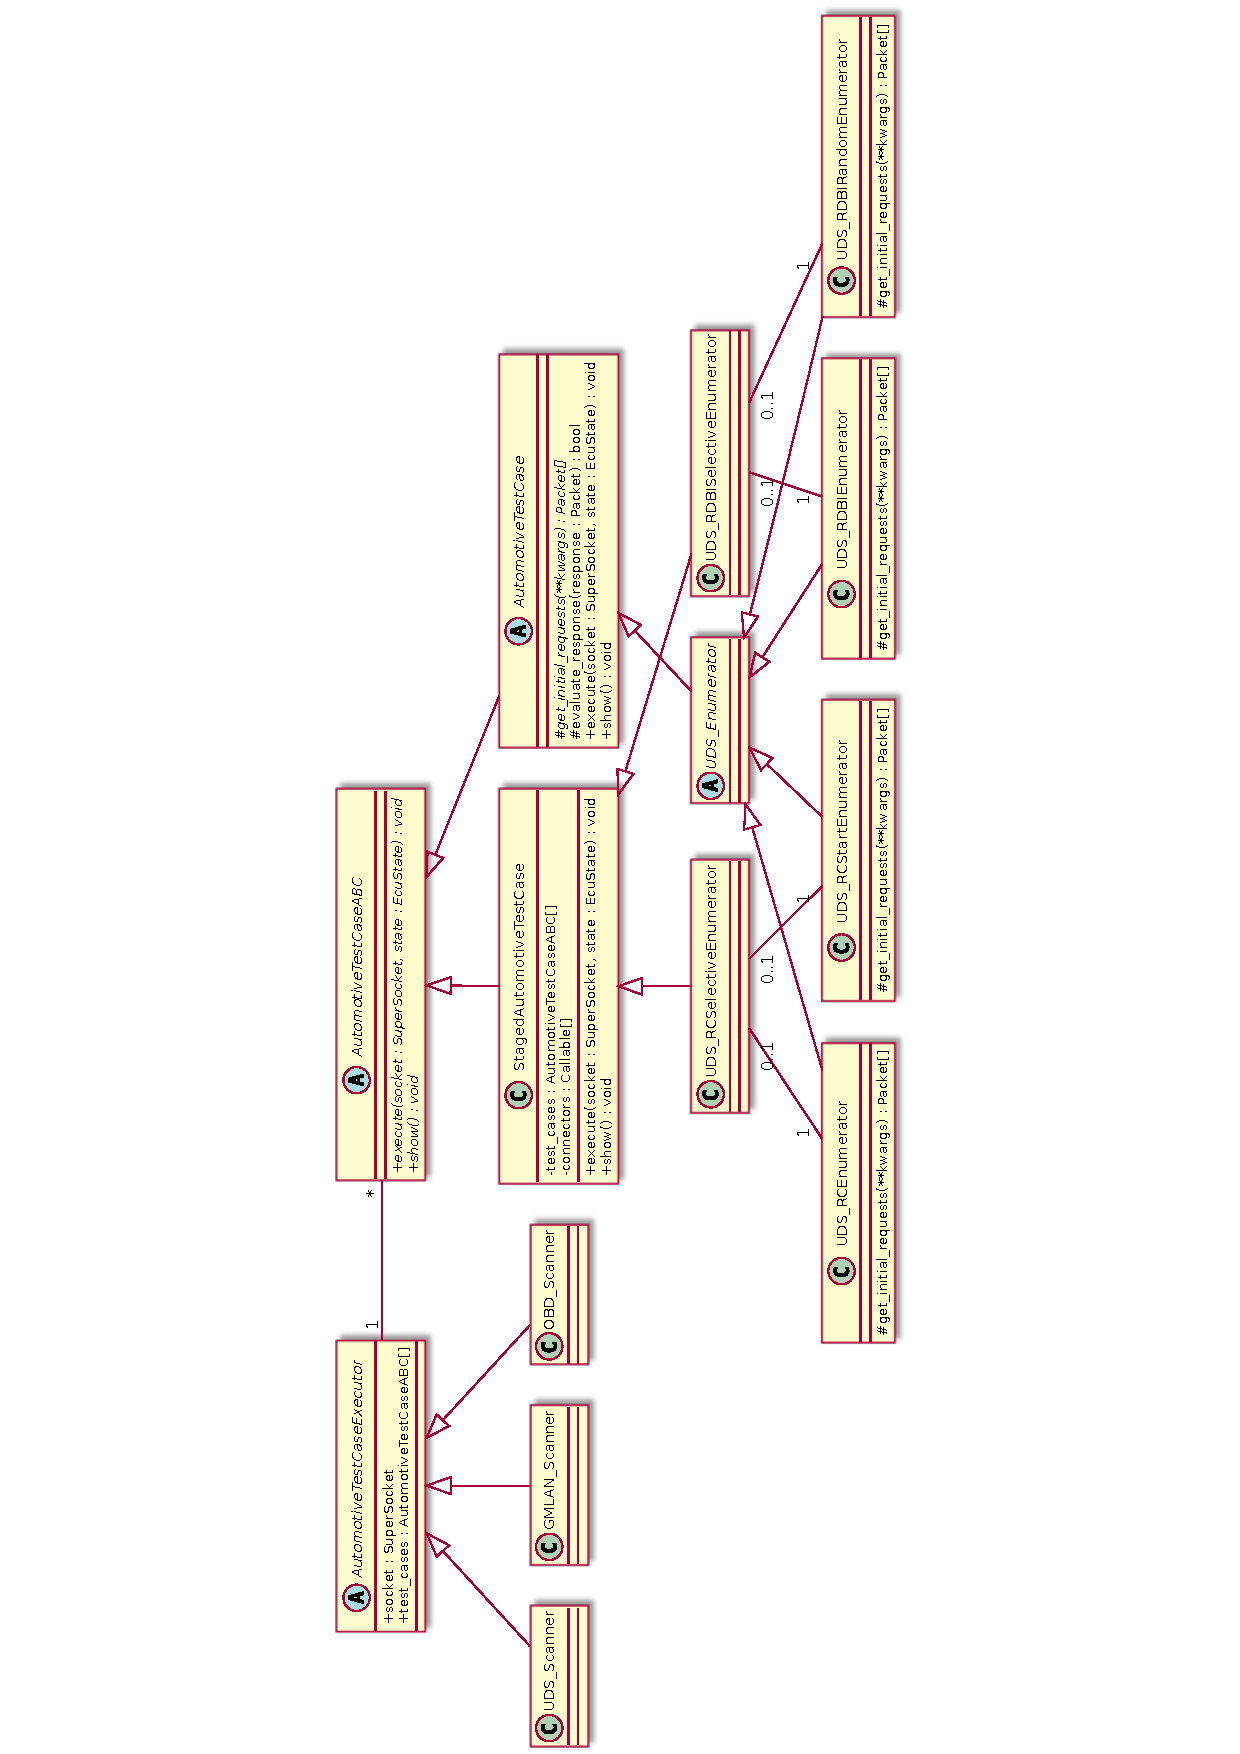
\includegraphics[height=0.9\textheight]{uml/overview}
\end{figure}

\chapter{First version of the RDBI Random enumerator}
\label{app:random-not-compact}

\begin{minted}
[frame=single,
framerule=0pt,
framesep=2mm,
baselinestretch=1.2,
bgcolor=VeryLightGray,
fontsize=\footnotesize,
linenos]
{python}
def _get_initial_requests(self, **kwargs):
    samples_per_block = [
        1, 0, 0, 0, 29, 22, 19, 0, 11, 11, 13, 14, 31, 4, 26, 1,
        30, 4, 20, 5, 49, 54,
        9, 4, 10, 8, 0, 0, 6, 3, 1, 0, 11, 0, 1, 0, 4, 3, 0, 1, 9,
        9, 3, 1, 2, 0, 0, 3,
        4, 3, 0, 0, 8, 0, 0, 0, 0, 0, 0, 0, 0, 0, 0, 0, 35, 0, 2,
        1, 24, 19, 30, 28,
        16, 4, 6, 27, 41, 11, 6, 0, 0, 2, 0, 1, 0, 0, 1, 0, 3, 0,
        2, 1, 16, 0, 0, 0, 0,
        15, 20, 0, 6, 5, 5, 10, 0, 1, 10, 0, 4, 0, 0, 0, 0, 0, 0,
        0, 0, 0, 0, 0, 0, 0,
        0, 0, 3, 0, 0, 0, 7, 0, 0, 0, 0, 0, 1, 0, 15, 14, 27, 10,
        0, 0, 0, 0, 0, 0, 1,
        0, 9, 0, 2, 0, 2, 0, 0, 0, 0, 0, 0, 0, 0, 1, 0, 0, 0, 0, 0,
        0, 23, 15, 16, 16,
        2, 0, 0, 0, 3, 4, 2, 1, 1, 0, 0, 0, 0, 0, 0, 2, 0, 0, 0, 0,
        0, 0, 0, 0, 0, 0,
        0, 0, 0, 0, 0, 0, 0, 0, 0, 0, 0, 0, 0, 0, 0, 0, 0, 0, 0, 0,
        0, 0, 0, 0, 0, 0,
        0, 0, 0, 0, 0, 0, 0, 0, 3, 0, 0, 2, 0, 0, 1, 0, 8, 0, 0, 0,
        1, 0, 0, 0, 0, 0,
        0, 0, 25, 0, 0, 0, 7, 2, 0, 0, 0, 1, 0, 1, 1, 0, 1, 0, 0,
        0, 0, 0, 0, 0, 0, 0,
        0, 0, 1, 0, 0, 0, 0, 0, 0, 0, 0, 6, 0, 0, 2, 0, 0, 1, 0, 0,
        0, 0, 0, 0, 0, 0,
        0, 0, 0, 0, 0, 0, 0, 0, 0, 0, 1, 1, 0, 1, 2, 1, 1, 3, 0, 0,
        0, 3, 19, 0, 2, 2,
        0, 0, 4, 10, 3, 0, 8, 0, 0, 1, 3, 0, 1, 0, 0, 0, 0, 0, 0,
        0, 0, 0, 0, 0, 1, 0,
        0, 0, 0, 0, 0, 0, 0, 0, 0, 0, 0, 0, 0, 0, 0, 0, 0, 0, 0, 0,
        0, 0, 0, 0, 0, 0,
        0, 0, 0, 0, 0, 0, 0, 0, 0, 0, 0, 0, 0, 0, 0, 0, 0, 0, 0, 0,
        0, 0, 0, 0, 0, 0,
        0, 0, 0, 0, 0, 0, 0, 0, 0, 0, 0, 0, 0, 0, 0, 0, 0, 0, 0, 0,
        0, 0, 0, 0, 0, 0,
        0, 0, 0, 0, 0, 0, 0, 0, 0, 0, 0, 0, 0, 0, 0, 0, 0, 0, 0, 0,
        0, 0, 0, 0, 0, 0,
        0, 0, 0, 0, 0, 0, 0, 0, 0, 0, 0, 0, 0, 0, 0, 0, 0, 0, 0, 0,
        0, 0, 0, 0, 0, 0,
        0, 0, 0, 0, 0, 0, 0, 0, 0, 0, 0, 0, 0, 0, 0, 0, 0, 0, 0, 0,
        0, 0, 0, 0, 0, 0,
        0, 0, 0, 0, 0, 0, 0, 0, 0, 0, 0, 0, 0, 0, 0, 0, 0, 0, 0, 0,
        0, 0, 0, 0, 0, 0,
        0, 0, 0, 0, 0, 0, 0, 0, 1, 0, 0, 0, 0, 0, 0, 0, 0, 0, 0, 0,
        0, 0, 0, 0, 0, 0,
        0, 0, 0, 0, 0, 0, 0, 0, 0, 0, 0, 0, 0, 0, 0, 0, 0, 0, 0, 0,
        0, 0, 0, 0, 0, 0,
        0, 0, 0, 0, 0, 0, 0, 0, 0, 0, 0, 0, 0, 0, 0, 0, 0, 0, 0, 0,
        0, 0, 0, 0, 0, 0,
        0, 0, 0, 0, 0, 0, 0, 0, 0, 0, 0, 0, 0, 0, 0, 0, 0, 0, 0, 0,
        0, 0, 0, 0, 0, 0,
        0, 0, 0, 0, 0, 0, 0, 0, 0, 0, 0, 0, 0, 0, 0, 0, 0, 0, 0, 0,
        0, 0, 0, 0, 0, 0,
        0, 0, 0, 0, 0, 0, 0, 0, 0, 0, 0, 0, 0, 0, 0, 0, 0, 0, 0, 0,
        0, 0, 0, 0, 0, 0,
        0, 0, 0, 0, 0, 0, 0, 0, 0, 0, 0, 0, 1, 0, 0, 0, 0, 0, 0, 0,
        0, 0, 0, 0, 0, 0,
        0, 0, 0, 0, 0, 0, 0, 0, 0, 0, 0, 0, 0, 0, 0, 0, 0, 0, 0, 0,
        0, 0, 0, 0, 0, 0,
        0, 0, 0, 0, 0, 0, 0, 0, 0, 0, 0, 0, 0, 0, 0, 0, 0, 0, 0, 0,
        0, 0, 0, 0, 0, 0,
        0, 0, 0, 0, 0, 0, 0, 0, 0, 0, 0, 0, 0, 0, 0, 0, 0, 0, 0, 0,
        0, 0, 0, 0, 0, 0,
        0, 0, 0, 0, 0, 0, 0, 0, 0, 0, 0, 0, 0, 0, 0, 0, 0, 0, 0, 0,
        0, 0, 0, 0, 0, 0,
        0, 0, 0, 0, 0, 0, 0, 0, 0, 0, 6, 2, 0, 0, 0, 0, 0, 0, 0, 0,
        0, 0, 0, 0, 0, 0,
        0, 0, 0, 0, 0, 0, 0, 0, 0, 0, 0, 0, 0, 0, 0, 0, 0, 0, 0, 0,
        0, 0, 0, 0, 0, 0,
        0, 0, 0, 0, 0, 0, 0, 0, 0, 0, 0, 0, 0, 0, 0, 0, 0, 0, 0, 0,
        0, 0, 0, 0, 0, 1,
        4, 0, 0, 0, 0, 0, 0, 0, 0, 0, 0, 0, 0, 0, 0, 0, 0, 0, 0, 0,
        0, 0, 0, 0, 0, 0,
        0, 0, 0, 0, 0, 0, 0, 0, 0, 0, 0, 0, 0, 0, 0, 0, 0, 0, 0, 0,
        0, 0, 0, 0, 0, 0,
        0, 0, 0, 0, 4, 0, 3, 1, 0, 0, 0, 0, 12, 13, 34, 3, 0, 0, 0,
        0, 10, 0, 0, 0, 0,
        0, 0, 0, 0, 0, 0, 0, 0, 0, 0, 0, 0, 0, 0, 0, 0, 0, 0, 0, 0,
        0, 0, 0, 3, 0, 0,
        0, 0, 0, 0, 0, 0, 0, 0, 0, 23, 14, 15, 0, 0, 0, 0, 0, 0, 0,
        0, 0]


    to_scan = []
    block_size = UDS_RDBIRandomEnumerator.block_size
    for block_index, start in enumerate(range(0, 2 ** 16, block_size)):
        end = start + block_size
        count_samples = max(probabilities[block_index] * block_size, 1)
        to_scan += random.sample(range(start, end), count_samples)

    # Remaining code did not change
    # [...]
\end{minted}


\end{document}
